%
%Не забыть:
%--------------------------------------
%Вставить колонтитулы, поменять название на титульнике



%--------------------------------------

\documentclass[a4paper, 12pt]{article} 

%--------------------------------------
%Russian-specific packages
%--------------------------------------
%\usepackage[warn]{mathtext}
\usepackage[T2A]{fontenc}
\usepackage[utf8]{inputenc}
\usepackage[english,russian]{babel}
\usepackage[intlimits]{amsmath}
\usepackage{esint}
%--------------------------------------
%Hyphenation rules
%--------------------------------------
\usepackage{hyphenat}
\hyphenation{ма-те-ма-ти-ка вос-ста-нав-ли-вать}
%--------------------------------------
%Packages
%--------------------------------------
\usepackage{amsmath}
\usepackage{amssymb}
\usepackage{amsfonts}
\usepackage{amsthm}
\usepackage{latexsym}
\usepackage{mathtools}
\usepackage{etoolbox}%Булевые операторы
\usepackage{extsizes}%Выставление произвольного шрифта в \documentclass
\usepackage{geometry}%Разметка листа
\usepackage{indentfirst}
\usepackage{wrapfig}%Создание обтекаемых текстом объектов
\usepackage{fancyhdr}%Создание колонтитулов
\usepackage{setspace}%Настройка интерлиньяжа
\usepackage{lastpage}%Вывод номера последней страницы в документе, \lastpage
\usepackage{soul}%Изменение параметров начертания
\usepackage{hyperref}%Две строчки с настройкой гиперссылок внутри получаеммого
\usepackage[usenames,dvipsnames,svgnames,table,rgb]{xcolor}% pdf-документа
\usepackage{multicol}%Позволяет писать текст в несколько колонок
\usepackage{cite}%Работа с библиографией
\usepackage{subfigure}% Человеческая вставка нескольких картинок
\usepackage{tikz}%Рисование рисунков
\usepackage{float}% Возможность ставить H в положениях картинки
\usepackage{mhchem}
% Для картинок Моти
\usepackage{misccorr}
\usepackage{lscape}
\usepackage{cmap}



\usepackage{graphicx,xcolor}
\graphicspath{{Pictures/}}
\DeclareGraphicsExtensions{.pdf,.png,.jpg}

%----------------------------------------
%Список окружений
%----------------------------------------
\newenvironment {theor}[2]
{\smallskip \par \textbf{#1.} \textit{#2}  \par $\blacktriangleleft$}
{\flushright{$\blacktriangleright$} \medskip \par} %лемма/теорема с доказательством
\newenvironment {proofn}
{\par $\blacktriangleleft$}
{$\blacktriangleright$ \par} %доказательство
%----------------------------------------
%Список команд
%----------------------------------------
\newcommand{\grad}
{\mathop{\mathrm{grad}}\nolimits\,} %градиент

\newcommand{\diver}
{\mathop{\mathrm{div}}\nolimits\,} %дивергенция

\newcommand{\rot}
{\ensuremath{\mathrm{rot}}\,}

\newcommand{\Def}[1]
{\underline{\textbf{#1}}} %определение

\newcommand{\RN}[1]
{\MakeUppercase{\romannumeral #1}} %римские цифры

\newcommand {\theornp}[2]
{\textbf{#1.} \textit{ #2} \par} %Написание леммы/теоремы без доказательства

\newcommand{\qrq}
{\ensuremath{\quad \Rightarrow \quad}} %Человеческий знак следствия

\newcommand{\qlrq}
{\ensuremath{\quad \Leftrightarrow \quad}} %Человеческий знак равносильности

\renewcommand{\phi}{\varphi} %Нормальный знак фи

\newcommand{\me}
{\ensuremath{\mathbb{E}}}

\newcommand{\md}
{\ensuremath{\mathbb{D}}}



%\renewcommand{\vec}{\overline}




%----------------------------------------
%Разметка листа
%----------------------------------------
\geometry{top = 3cm}
\geometry{bottom = 2cm}
\geometry{left = 1.5cm}
\geometry{right = 1.5cm}
%----------------------------------------
%Колонтитулы
%----------------------------------------
\pagestyle{fancy}%Создание колонтитулов
\fancyhead{}
%\fancyfoot{}
%----------------------------------------
%Интерлиньяж (расстояния между строчками)
%----------------------------------------
%\onehalfspacing -- интерлиньяж 1.5
%\doublespacing -- интерлиньяж 2
%----------------------------------------
%Настройка гиперссылок
%----------------------------------------
\hypersetup{				% Гиперссылки
	unicode=true,           % русские буквы в раздела PDF
	pdftitle={Заголовок},   % Заголовок
	pdfauthor={Автор},      % Автор
	pdfsubject={Тема},      % Тема
	pdfcreator={Создатель}, % Создатель
	pdfproducer={Производитель}, % Производитель
	pdfkeywords={keyword1} {key2} {key3}, % Ключевые слова
	colorlinks=true,       	% false: ссылки в рамках; true: цветные ссылки
	linkcolor=blue,          % внутренние ссылки
	citecolor=blue,        % на библиографию
	filecolor=magenta,      % на файлы
	urlcolor=red           % на URL
}
%----------------------------------------
%Работа с библиографией (как бич)
%----------------------------------------
\renewcommand{\refname}{Список литературы}%Изменение названия списка литературы для article
%\renewcommand{\bibname}{Список литературы}%Изменение названия списка литературы для book и report
%----------------------------------------
\begin{document}
	\begin{titlepage}
		\begin{center}
			$$$$
			$$$$
			$$$$
			$$$$
			{\Large{НАЦИОНАЛЬНЫЙ ИССЛЕДОВАТЕЛЬСКИЙ УНИВЕРСИТЕТ}}\\
			\vspace{0.1cm}
			{\Large{ВЫСШАЯ ШКОЛА ЭКОНОМИКИ}}\\
			\vspace{0.25cm}
			{\large{Факультет физики}}\\
			\vspace{5.5cm}
			{\Huge\textbf{{Серия лабораторных работ по современной физике}}}\\%Общее название
			\vspace{1cm}
			{Работу выполнили студенты 3 курса}\\
			{Захаров Сергей Дмитриевич}\\
			{Еремин Валентин Антонович}\\
			\vfill
			
\includegraphics[width = 0.2\textwidth]{HSElogo}\\
			\vfill
			Москва\\
			2021
		\end{center}
	\end{titlepage}
	
\tableofcontents

\newpage

\section{Спектрометр}
\fancyhead[R]{\textsc{Спектрометр}}%Вставить колонтитул сюда

\subsection{Постановка целей работы}

\begin{enumerate}
	\item Сборка спектрометра на основе дифракционной решетки.
	
	\item Получение спектров пропускания различных растворов и фотонных кристаллов.
	
\end{enumerate}

\subsection{Описание установки}

Установка была собрана с использованием линз с различной оптической силой, поляризаторов, щели, дифракционной решетки и камеры. Схема приведена на рисунке (\ref{fig:scheme})

\begin{figure}[H]
	\centering
	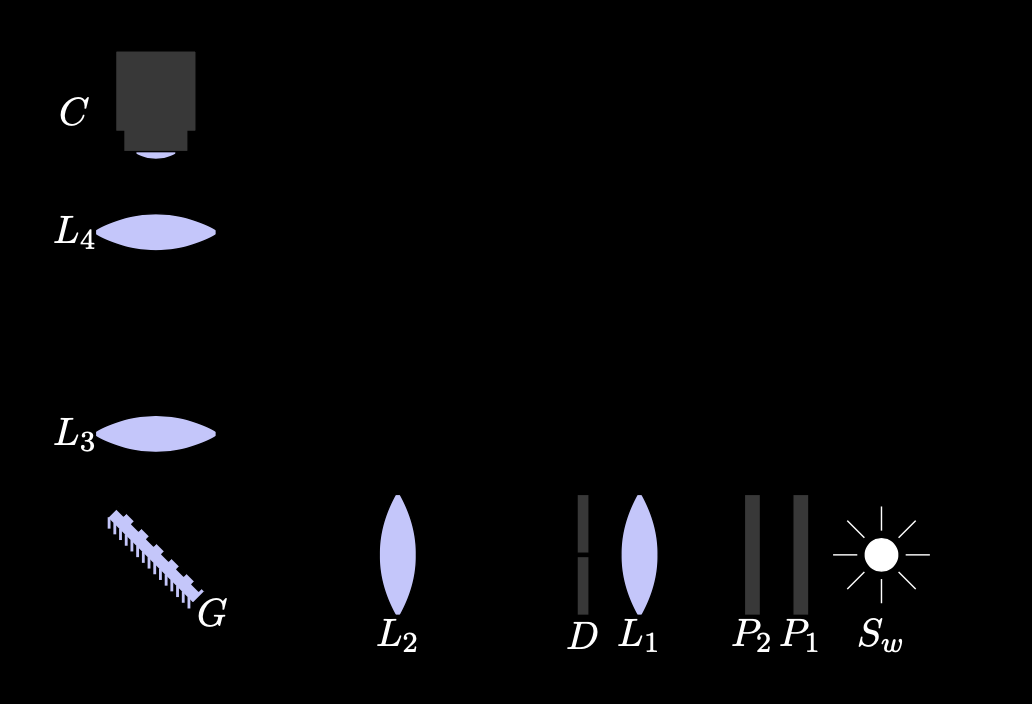
\includegraphics[width=0.7\linewidth]{Scheme.png}
	\caption{Схема установки.$P_1$ и $P_2$ - пара поляризаторов, источник находится в фокусе $L_1$, щель $D$ распложена в фокусе линзы $L_2$, $G$ - дифракционная решетка, $L_3$ и $L_4$ - линзы собирающие спектры на матрицу.}
	\label{fig:scheme}
\end{figure}

Таким образом на щель $D$ падал параллельный пучок. Расположение $D$ в фокусе $L_2$ в свою очередь позволяло получить параллельный пучок на дифракционной решетке, после чего регистрировался спектр.

\subsection{Калибровка матрицы}

Чтобы получить реальные значения зависимости интенсивности от длины волны, снимаемой с RGB матрицы, требуются реперные значение длин волн и соответсвующие им у.е., выдаваемые камерой. Для этого были использованы красный и зеленый лазеры, и в предположении, что зависимость линейная, получены абсолютные значения.

Здесь надо оговориться, что даже незначительная переюстировка системы приводила к ощутимым сдвигам спектра, поэтому к приведенным ниже данным следует относиться как к качественному анализу.


\subsection{Спектр пропускания}
Спектром пропускания образца называется спектральная зависимость (функция длины волны) его коэффициента пропускания. Коэффициентом пропускания называется отношение интенсивностей прошедшего через образец и падающего на образец излучения.

Спектр пропускания получался установкой образца на пути параллельных лучей перед дифракционной решеткой. Измереннные спектры различных растворов нормировались на пустую кювету.

\subsection{Фотонные кристаллы}

Фотонный кристалл - материал, структура которого характеризуется переодическим изменением диэлектрической проницаемости. 

Аналогично запрещенным и разрешенным энергетическим зонам в диэлектриках, в фотонных кристаллах будут возникать частотные зоны, нахождение фотона в которых невозможно. Дисперсия фотонов и электронов в переодической структуре приведена на картинке (\ref{fig:bandgap})

\begin{figure}[H]
	\centering
	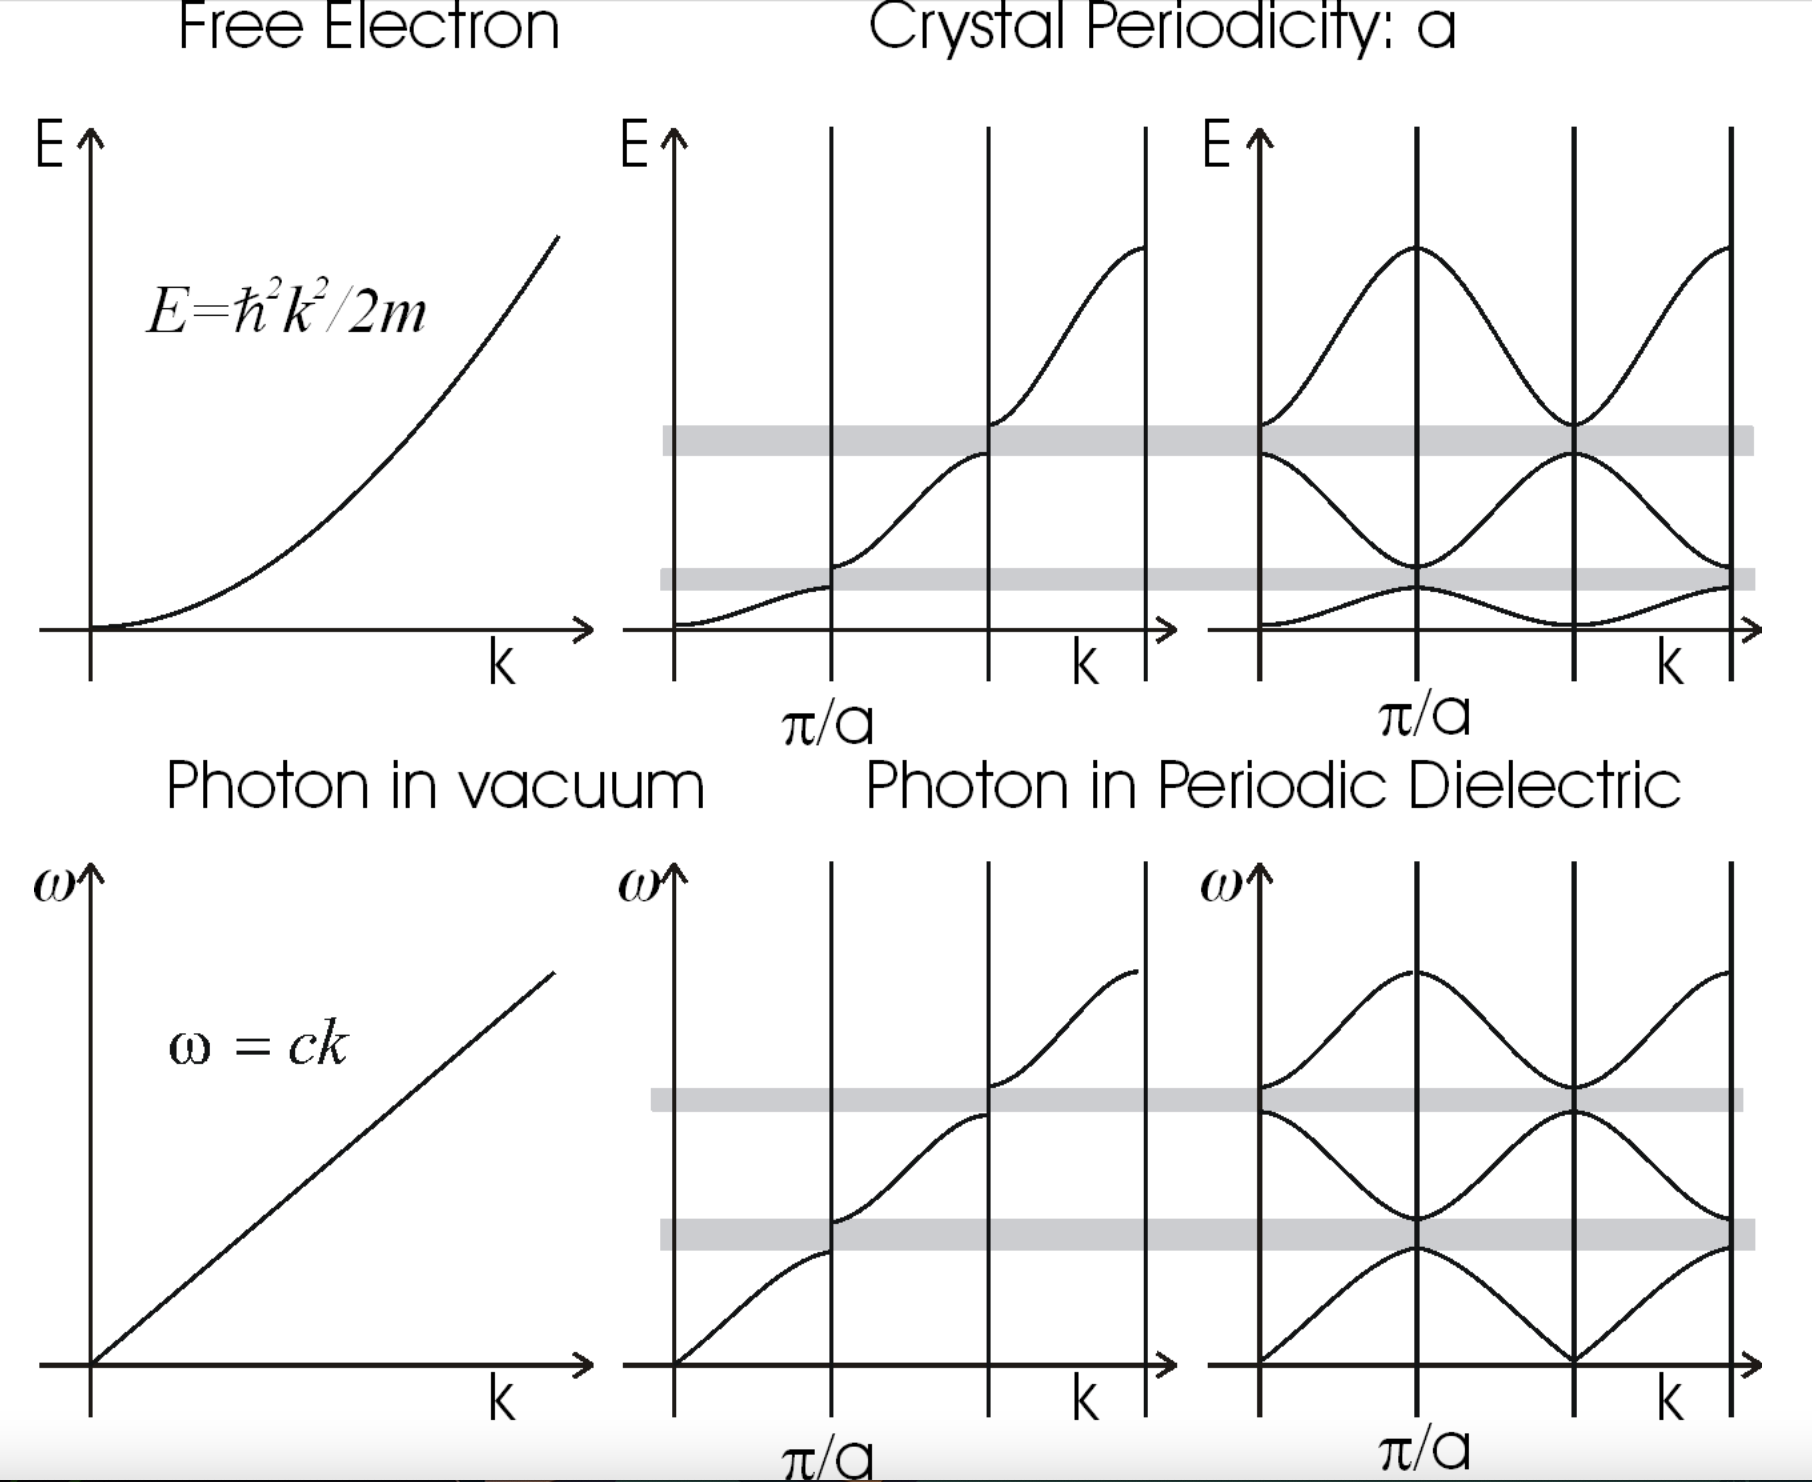
\includegraphics[width=0.7\linewidth]{bandgap.png}
	\caption{Дисперсия свободных фотонов и электронов и она же в переодическом потенциале после учета взаимодействия}
	\label{fig:bandgap}
\end{figure}

Важным различием между зонными теориями для электронов и фотонных кристаллов является в случае с фотонами учитывать также поляризацию соответствующих им волн. Это в свою очередь будет влиять на зависимость спектра пропускания для фотонных кристаллов от угла падения света.

\section{Обработка результатов}

В общей части сразу же отметим то, каким образом данные с трех каналов (красного, зеленого и синего) матрицы камеры складывались в одно целое. Сигнал от каждого из каналов пропорционален интенсивности, поэтому сложение сигналов производилось по формуле \ref{eq:main}:

\begin{equation}
	I_\Sigma = \left(\sqrt{I_\text{red}} + \sqrt{I_\text{green}} + \sqrt{I_\text{blue}}\right) ^ 2
	\label{eq:main}
\end{equation}

\subsection{Масштабирование шкалы камеры. Красный и синий лазеры}

Регистрация спектра производилась с помощью RGB-матрицы камеры. Для того, чтобы по фотографии спектра было возможно определить длину волны в любой части спектра, необходимо произвести калибровку. Для этого были взяты два лазера с известными с хорошей точностью длинами волн: синий с длиной волны 405~нм и красный гелий-неоновый лазер с длиной волны 632.8~нм. После этого шкала была линейно откалибрована так, чтобы пикам красного и синего лазеров соответствовали указанные длины волн. Спектры лазеров (с учетом откалиброванной шкалы) представлены на рисунках \ref{fig:redlaser}, \ref{fig:bluelaser}.

\begin{figure}[H]
	\centering
	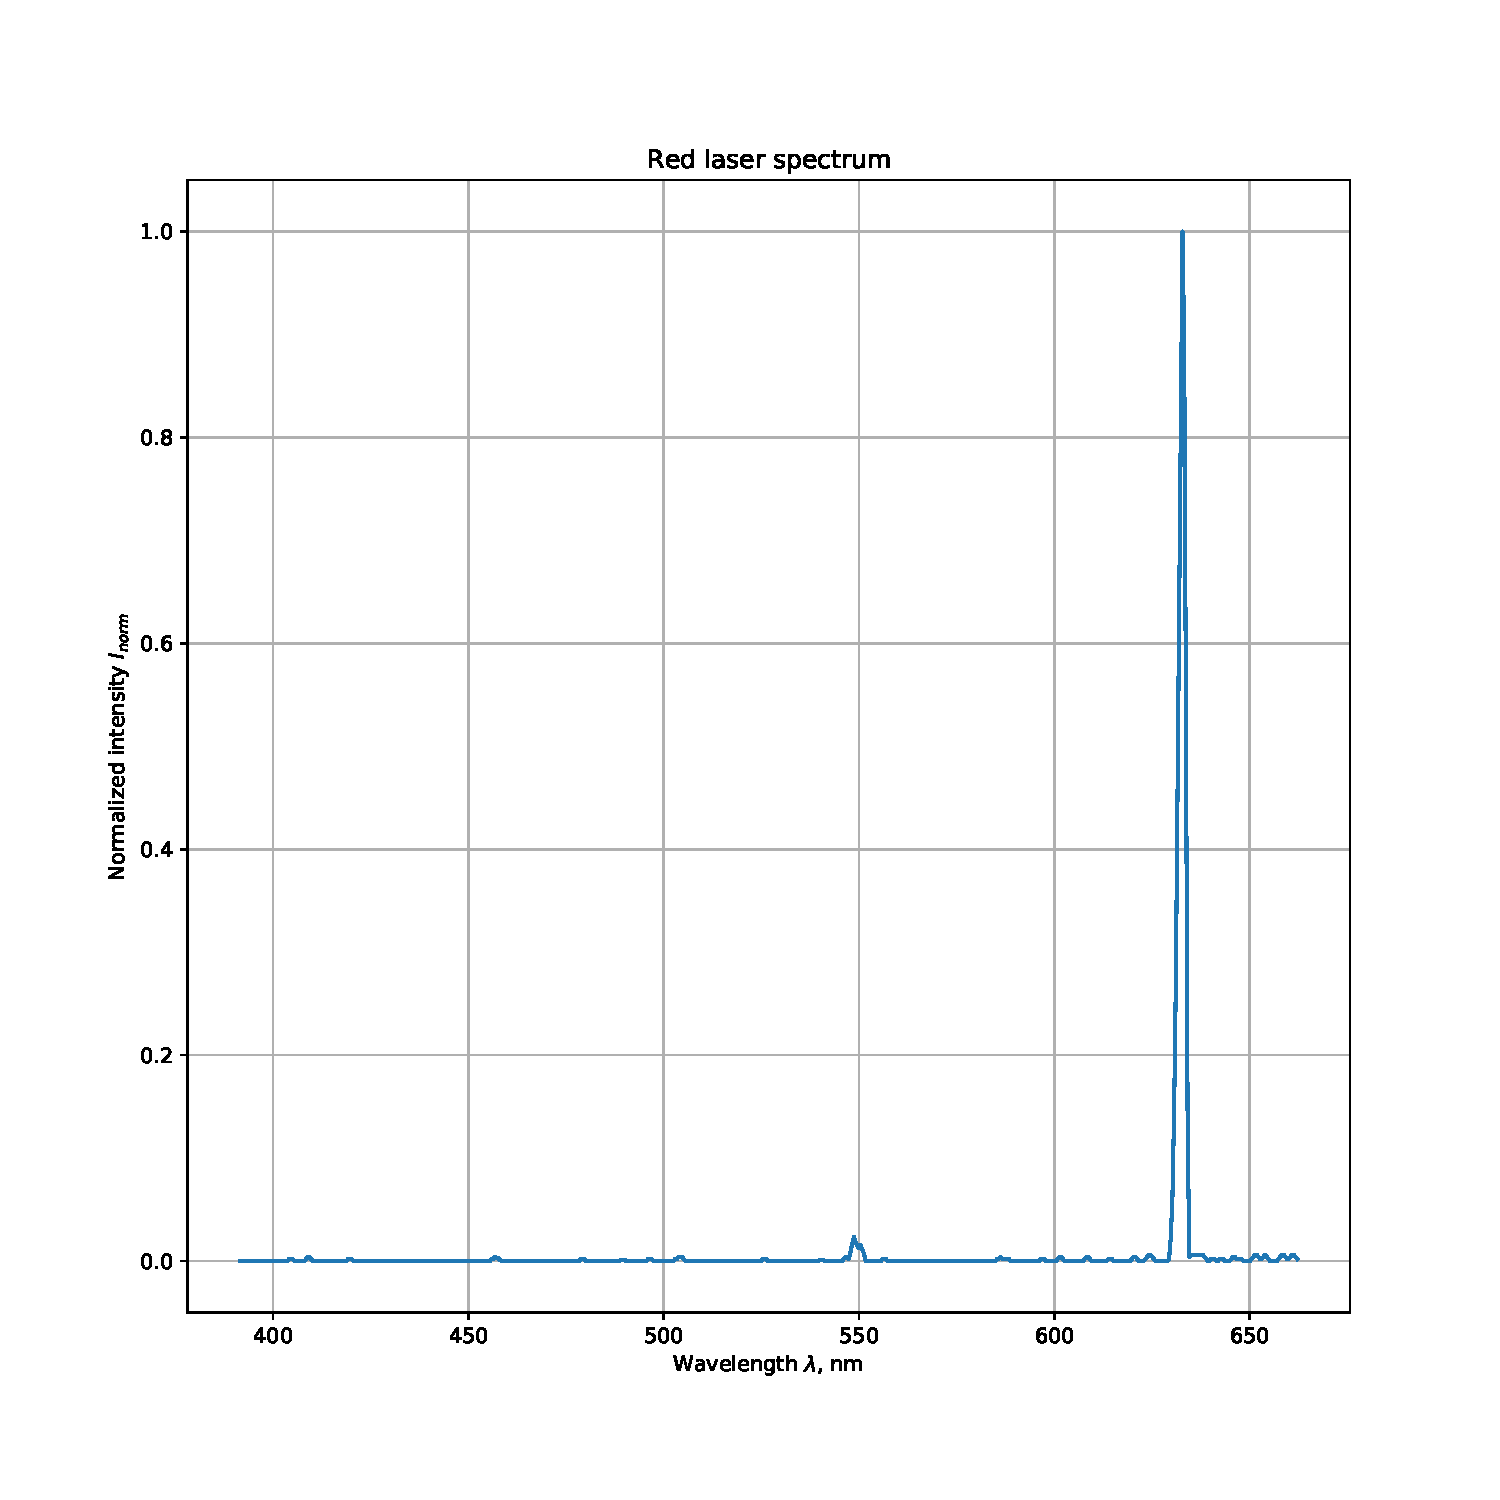
\includegraphics[width=0.7\linewidth]{redlaser}
	\caption{Откалиброванная длина волны красного лазера}
	\label{fig:redlaser}
\end{figure}

\begin{figure}[H]
	\centering
	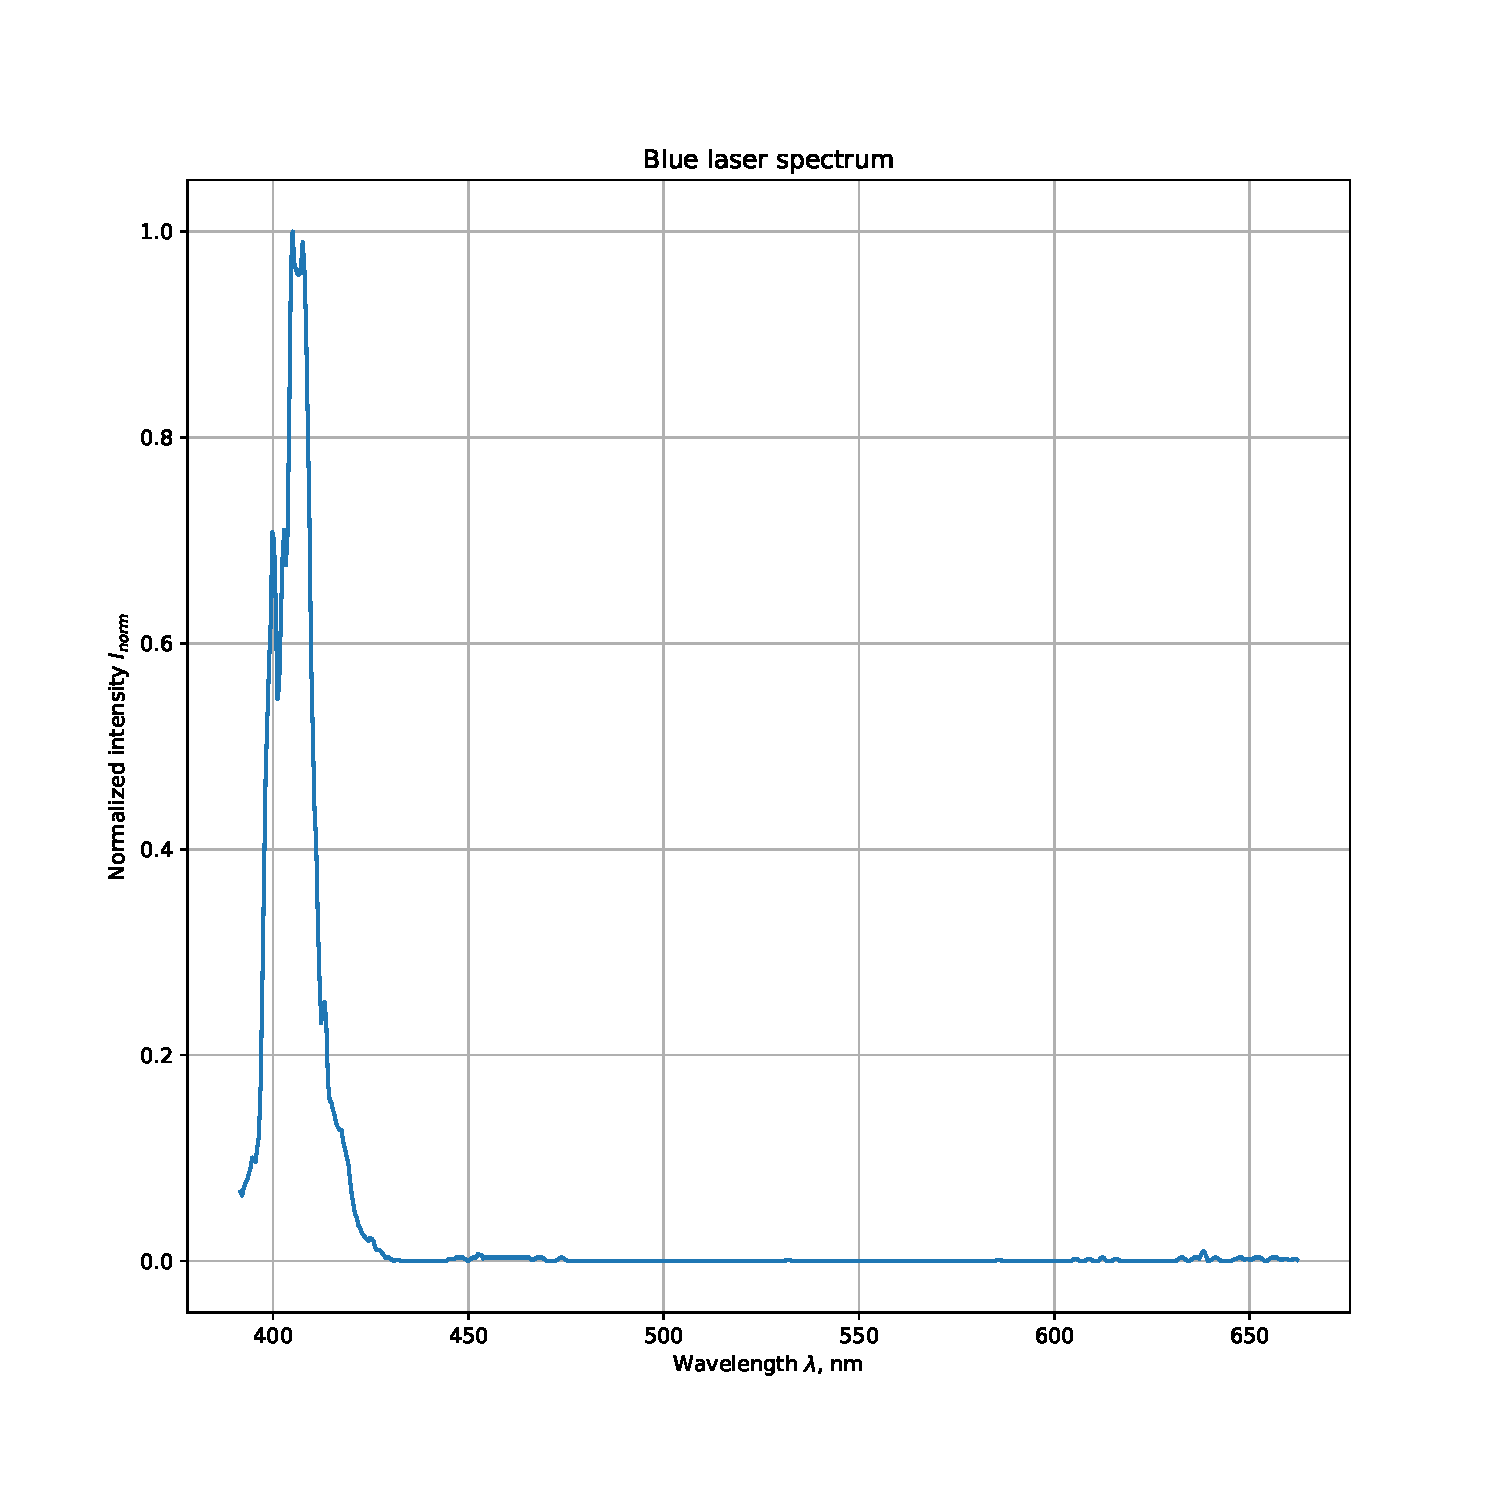
\includegraphics[width=0.7\linewidth]{bluelaser}
	\caption{Откалиброванная длина волны синего лазера }
	\label{fig:bluelaser}
\end{figure}

\subsection{Спектры пропускания различных растворов}

Имея откалиброванный на лазерах спектрометр можно получить спектры пропускания различных растворов, что и было сделано. Для этого сперва был получен спектр света светодиода после прохождения им пустой кюветы, в которую затем наливались различные исследуемые растворы. В экспериментах, однако, была допущена ошибка: между снятиями данных по различным растворам изменялась интенсивность света от светодиода (посредством изменения угла между главными направлениями поляризаторов), поэтому оказалось невозможным получить абсолютные значения спектров пропускания. Тем не менее, это упущение не влияет на саму форму спектра, что делает данные пригодными для анализа.

\subsubsection{CoCl$_3$}

Раствор \ce{CoCl3} --- зеленовато-желтого цвета, что позволяет нам ожидать максимума пропускания где-то в районе длины волны зеленого цвета, что и получилось на рисунке \ref{fig:cocl3}.


\begin{figure}[H]
	\centering
	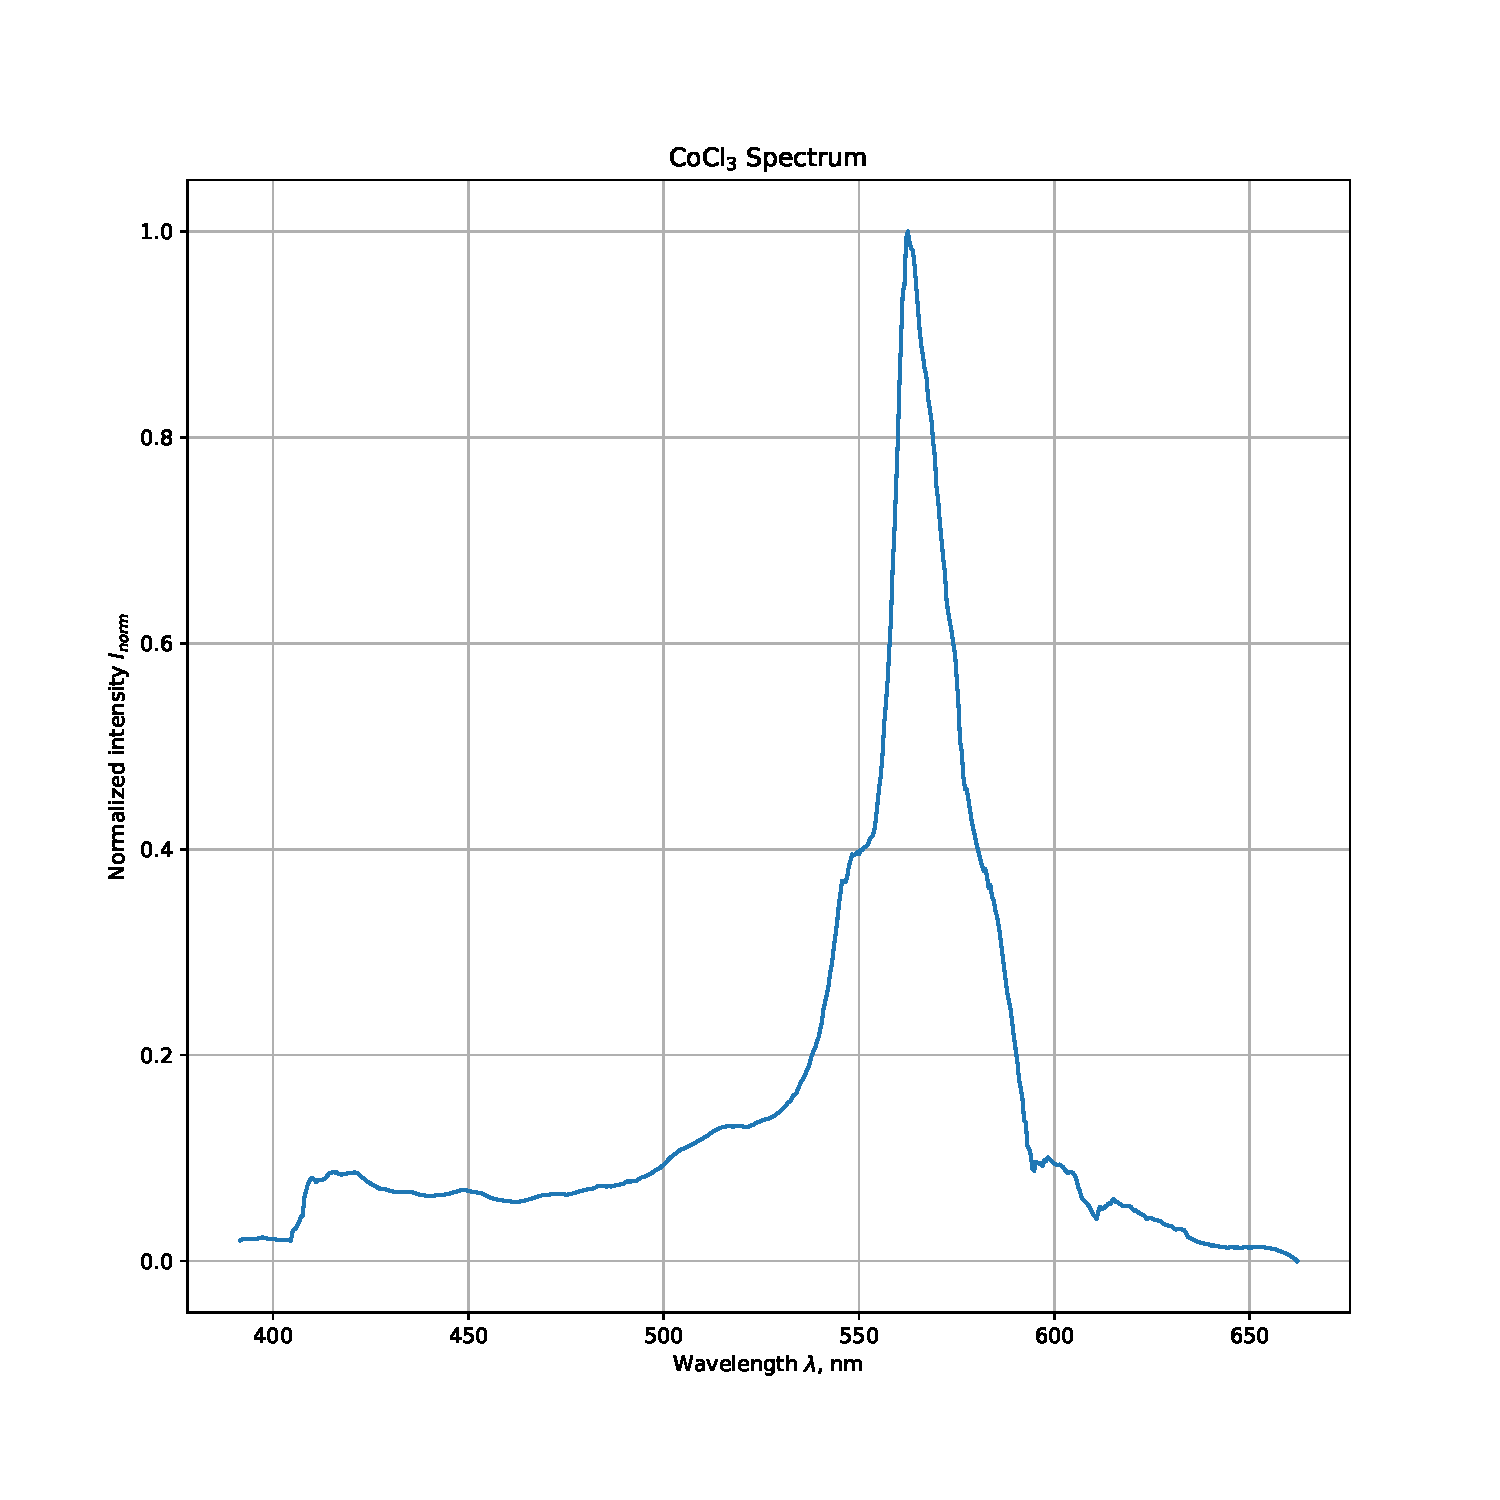
\includegraphics[width=0.7\linewidth]{cocl3.pdf}
	\caption{Спектр \ce{CoCl3}}
	\label{fig:cocl3}
\end{figure}

\subsubsection{CuSO$_4$}

Раствор \ce{CuSO4} --- сине-зеленого цвета, поэтому логичным ожиданием будет наличие пиков в районе синего и зеленого цветов. В принципе, это и получилось на экспериментальных данных (см. рисунок \ref{fig:cuso4}). Тем не менее, не до конца ясна причина столь низкого пропускания на частотах 450~нм --- 500~нм.

\begin{figure}[H]
	\centering
	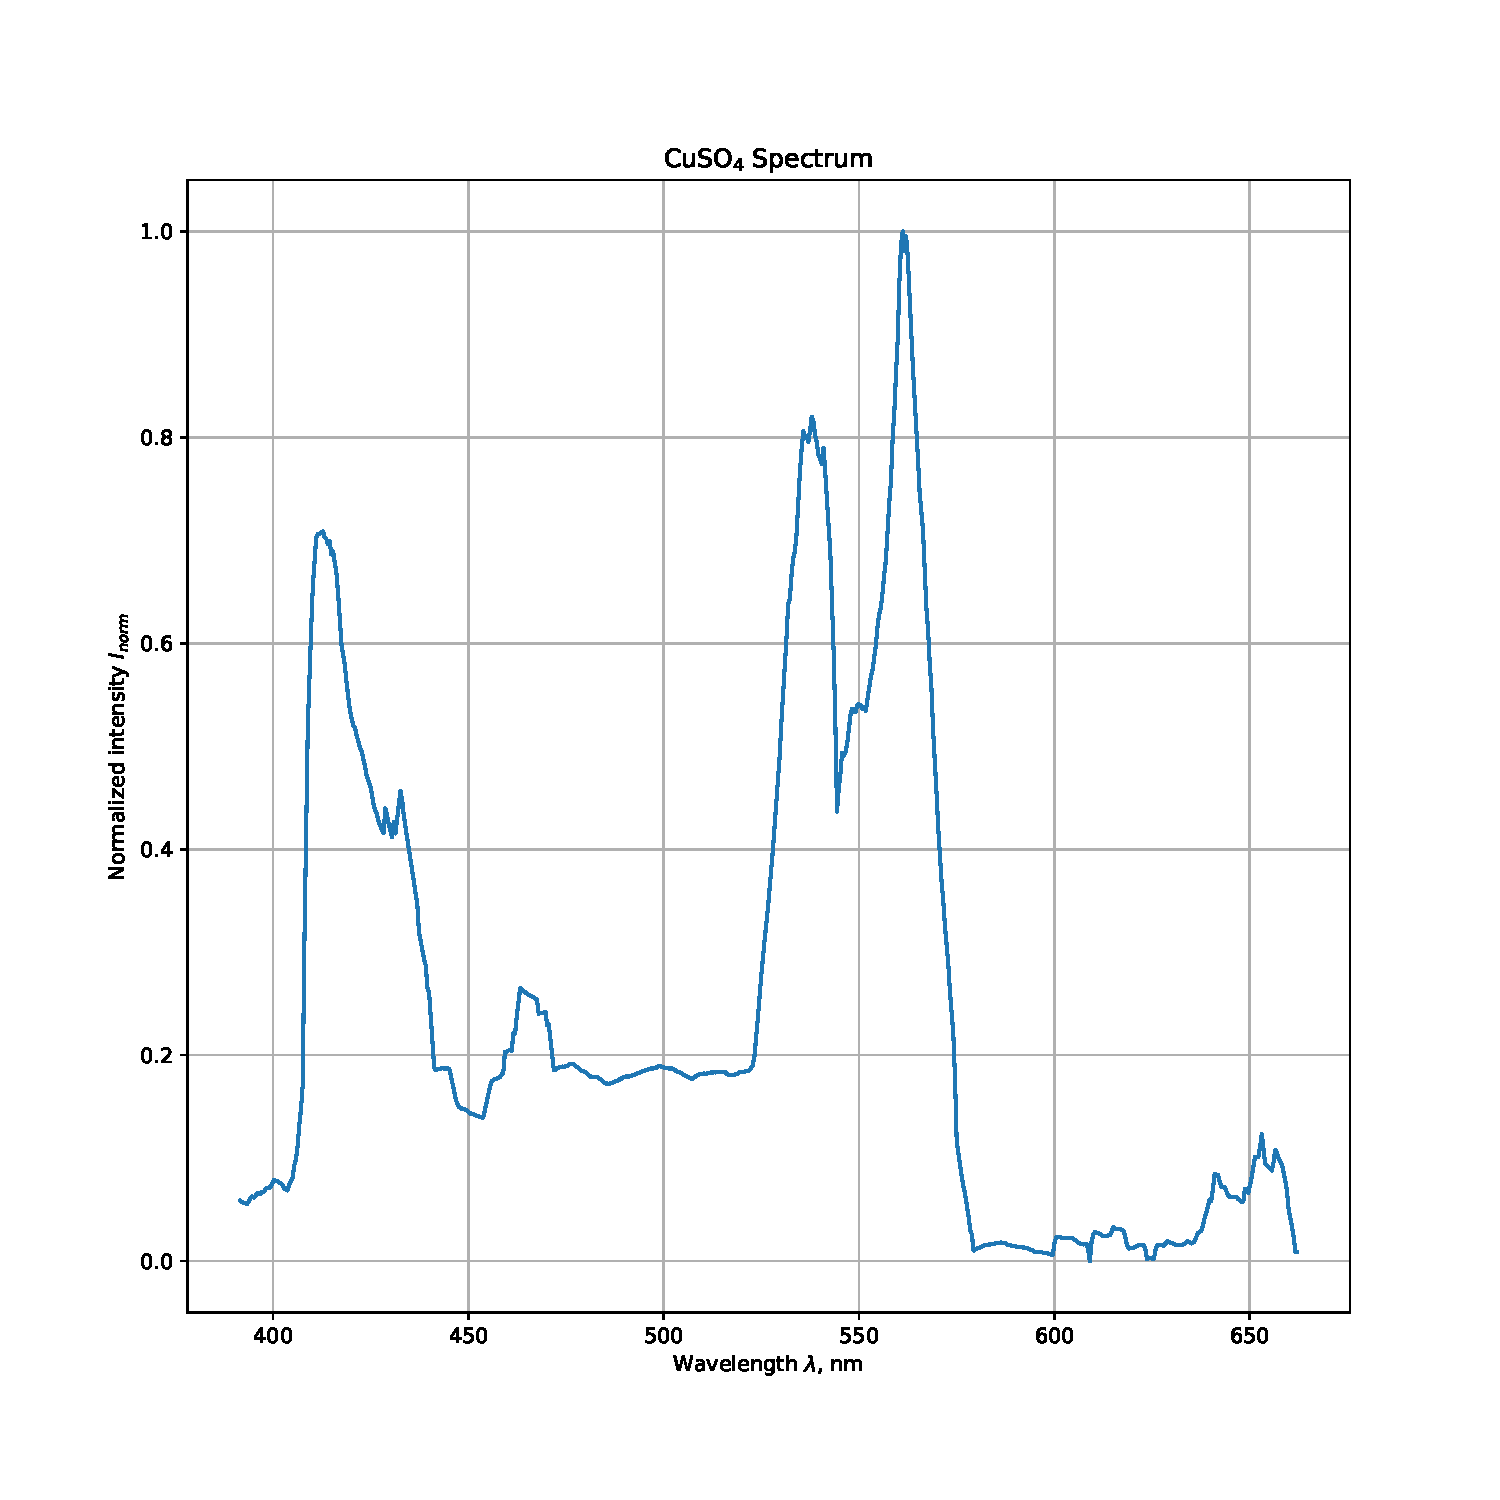
\includegraphics[width=0.7\linewidth]{cuso4.pdf}
	\caption{Спектр \ce{CuSO4}}
	\label{fig:cuso4}
\end{figure}

\subsubsection{Флуоресцеин}

Раствор флуоресцеина при освещении светом светодиода приобретает яркий кислотно-зеленый цвет. Было проведено две серии экспериментов: с обычным раствором и с разбавленным в два раза. Во втором случае цвет раствора оказывался более тусклым и каким-то более желтым, чем в первом. Результаты приведены на рисунках \ref{fig:fluorescein} и \ref{fig:fluorescein0.5}. Результаты эксперимента коррелируют с наблюдениями: в случае разбавленного раствора пропускание в зеленой области меньше, чем в случае неразбавленного.

\begin{figure}[H]
	\centering
	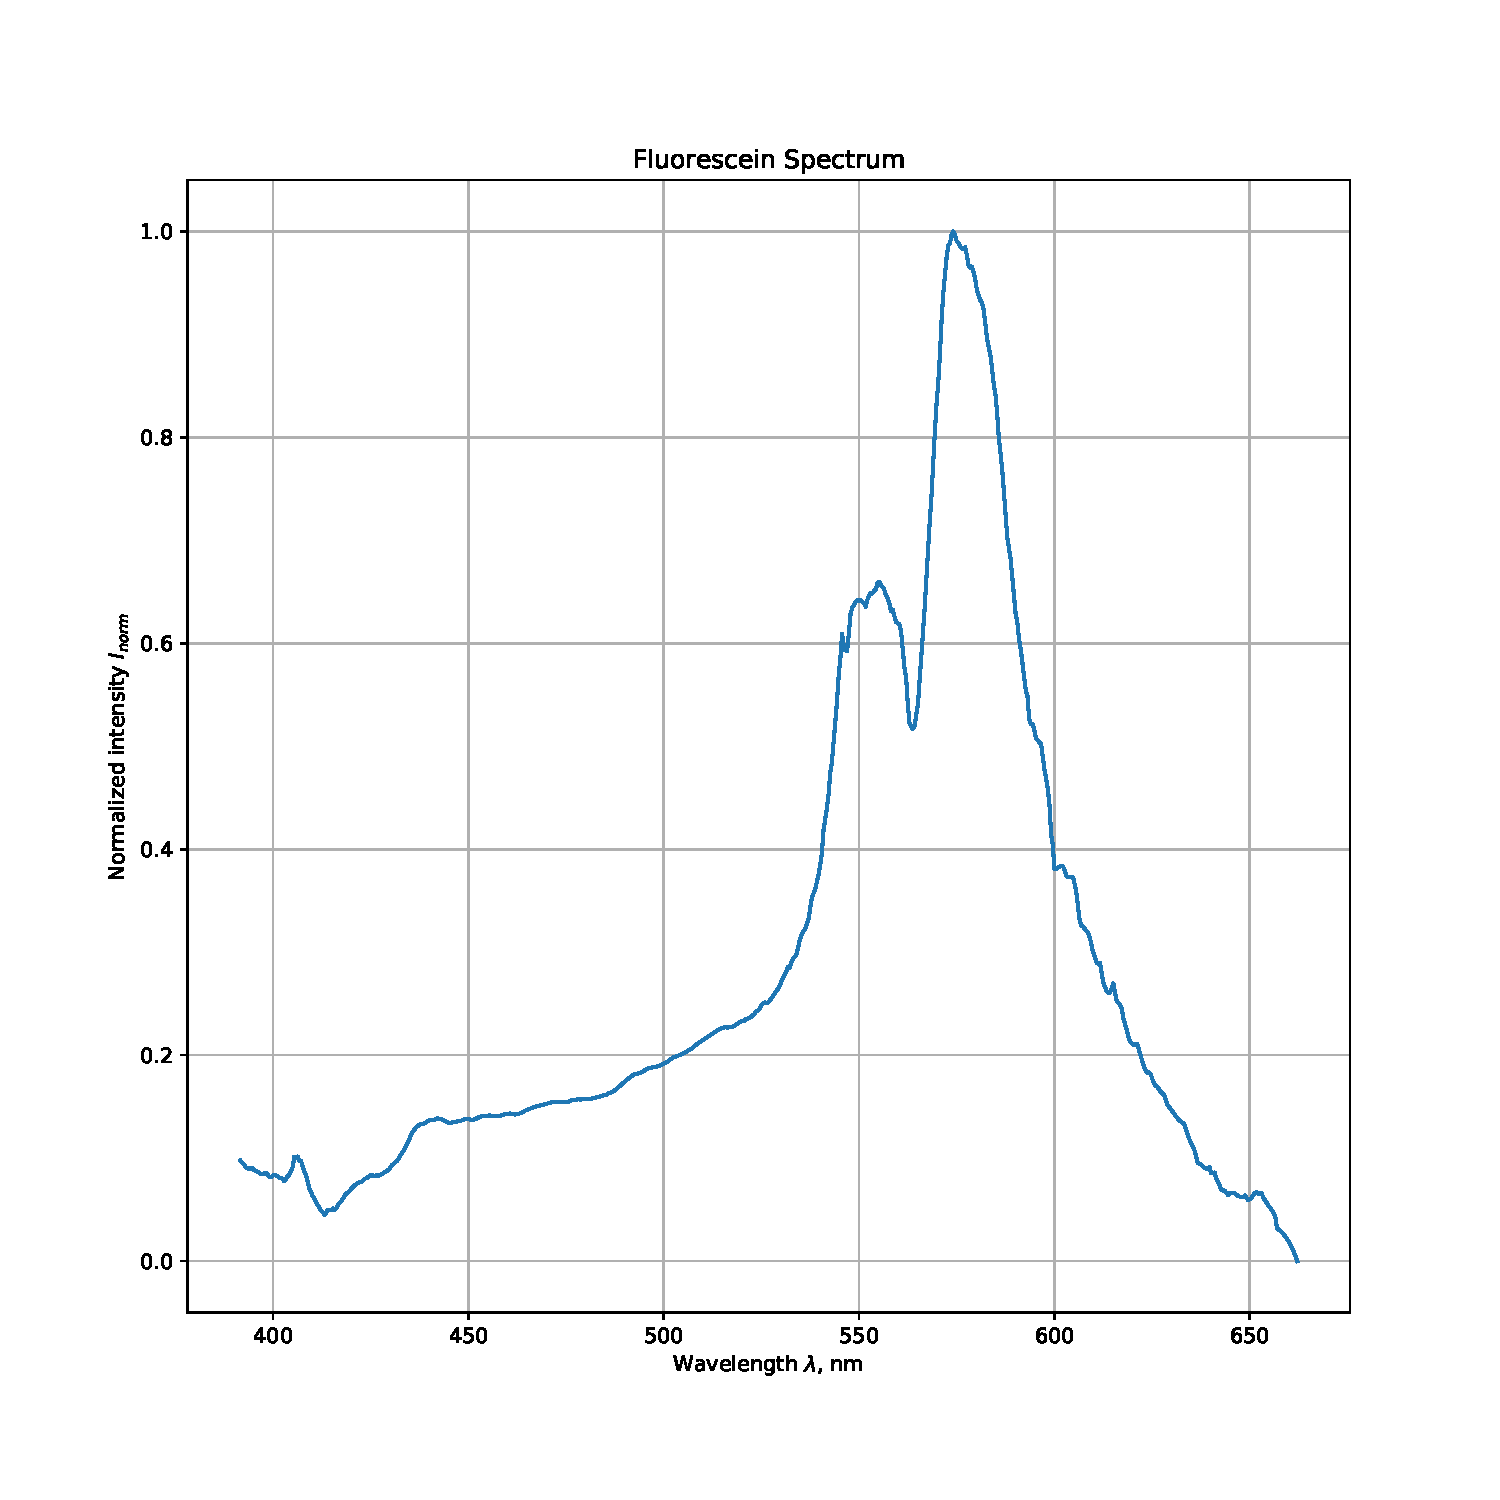
\includegraphics[width=0.7\linewidth]{c_yellow.pdf}
	\caption{Спектр флуоресцеина}
	\label{fig:fluorescein}
\end{figure}

\begin{figure}[H]
	\centering
	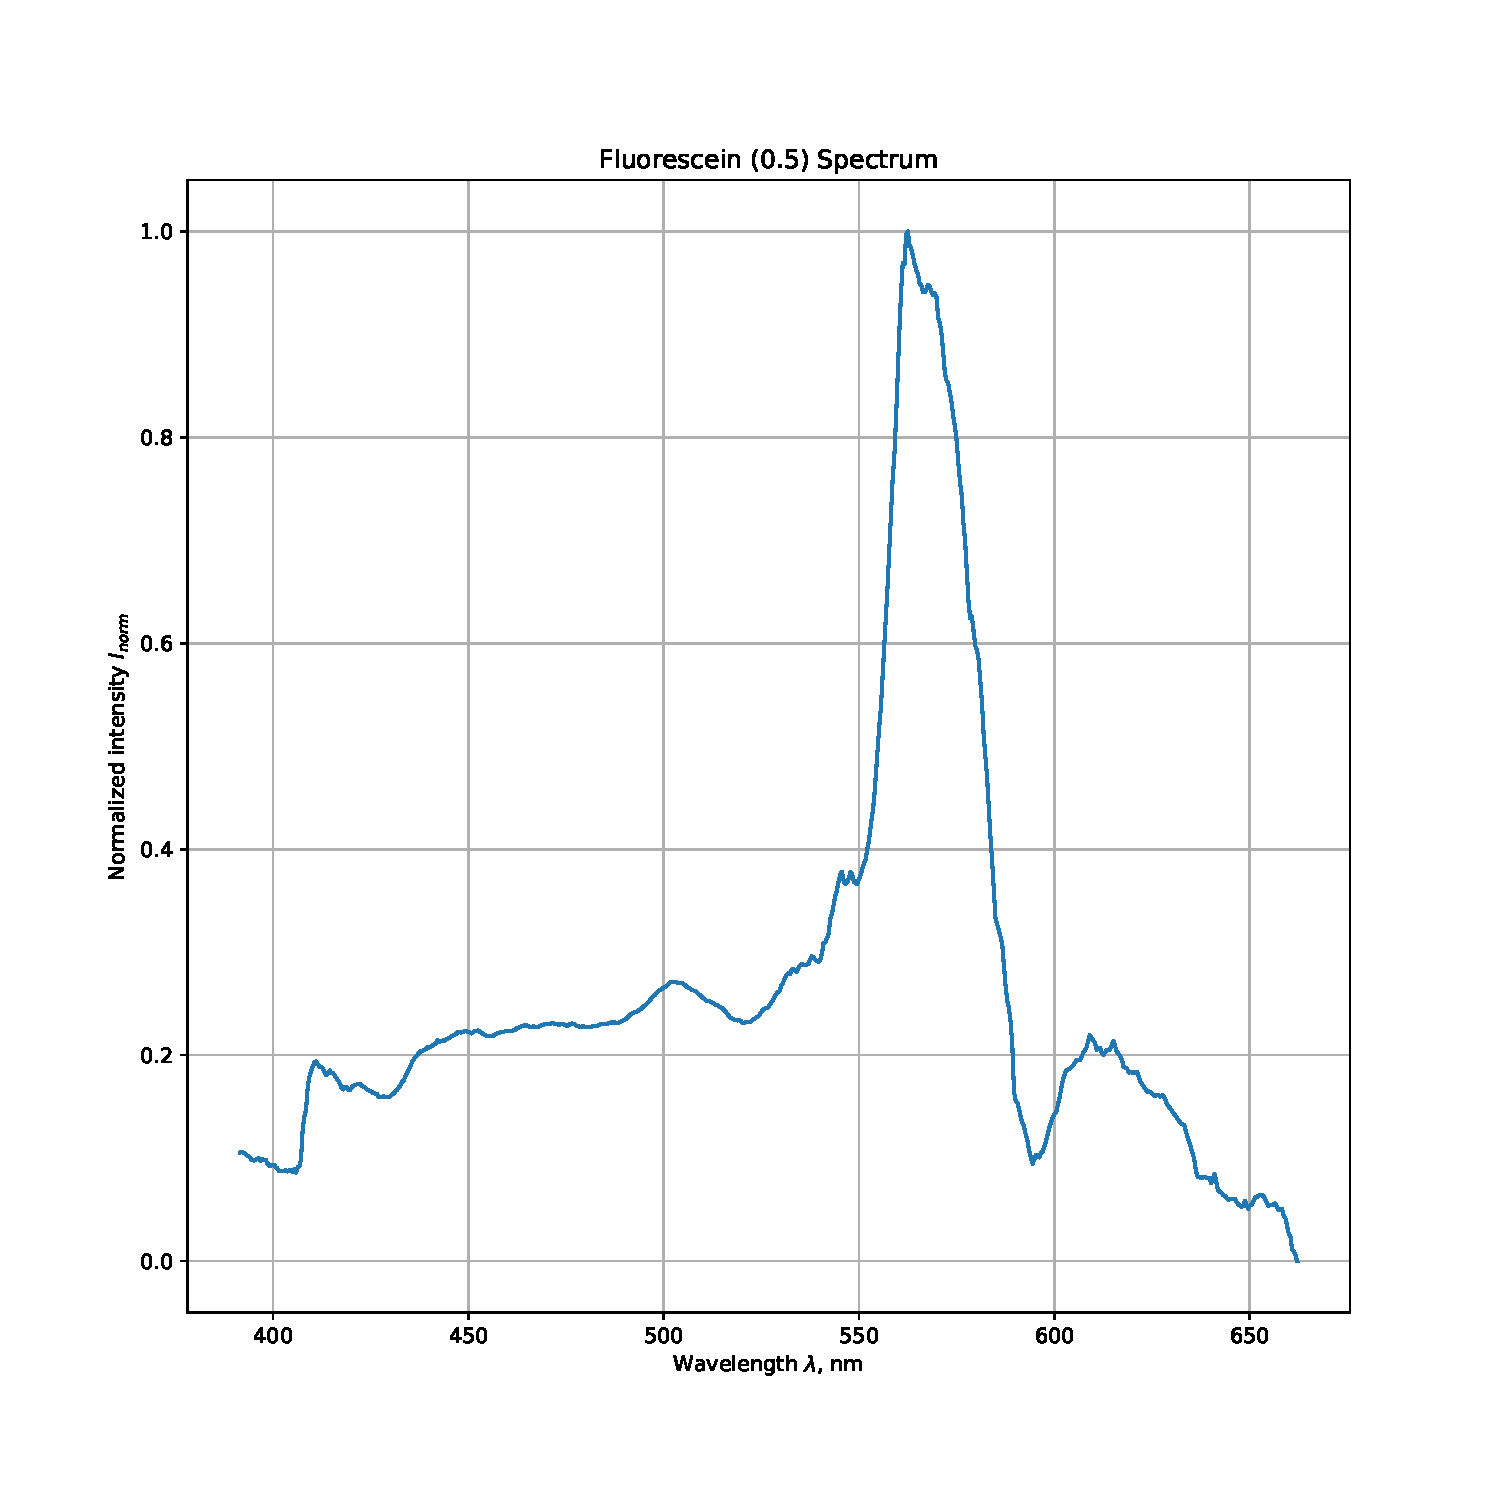
\includegraphics[width=0.7\linewidth]{c_lime.pdf}
	\caption{Спектр флуоресцина с уменьшенной вдвое концентрацией}
	\label{fig:fluorescein0.5}
\end{figure}

\subsubsection{K$_2$Cr$_2$O$_7$}

Раствор \ce{K2Cr2O7} --- красно-рыжего цвета, из-за чего предполагается наличие максимума в районе 600~нм и ближе к 700~нм. Тем не менее, экспериментальные данные демонстрируют нам пик в районе 560~нм (см. рисунок \ref{fig:k2cr2o7}), что не вяжется с цветом раствора. Возможное объяснение этому --- небрежность проведения этого эксперимента: поскольку данный спектр снимался последним, вполне допустимо, что к этому моменту калибровка спектрометра могла быть нарушена из-за постоянной активности вблизи него.

\begin{figure}[H]
	\centering
	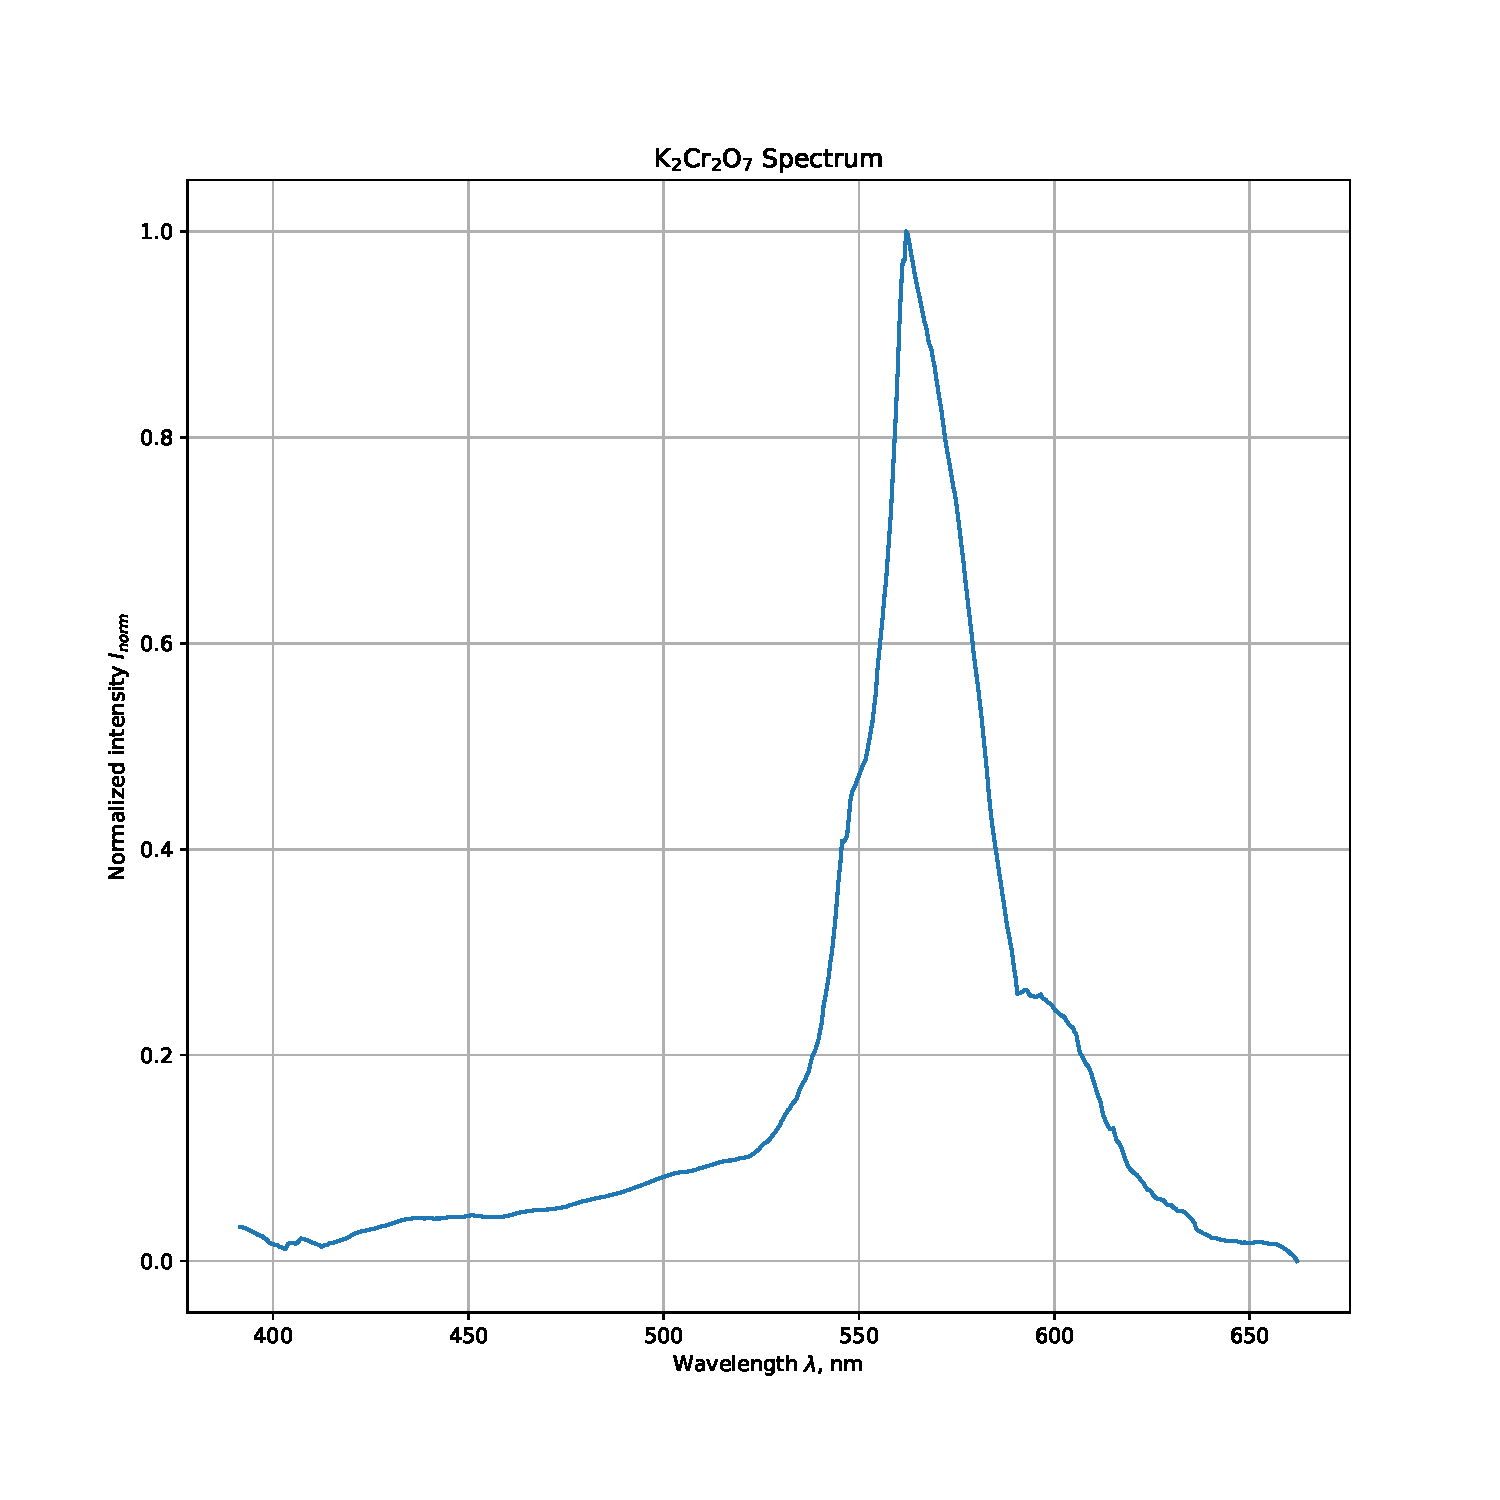
\includegraphics[width=0.7\linewidth]{k2cr2o7.pdf}
	\caption{Спектр \ce{K2Cr2O7}}
	\label{fig:k2cr2o7}
\end{figure}

\subsection{Фотонные кристаллы. Зависимость от угла}

Общая вводная про фотонные кристаллы была дана ранее. В экспериментах было взято 5 пластинок, каждая из которых была проснята в трех различных положениях: когда свет падает на нее перпендикулярно, под углом 30$^\circ$ и под углом 45$^\circ$. Результаты для различных пластинок представлены на рисунках ниже. Также для каждой из них добавлен исходный снятый спектр светодиода для сравнения.

Видно, что кое-где интенсивность после прохождения фотонного кристалла оказывалась местами больше, чем просто от светодиода. Логичным объяснением тут будет просто погрешность эксперимента. Отметим, однако, что в большинстве случаев превышения незначительные.

\begin{figure}[H]
	\centering
	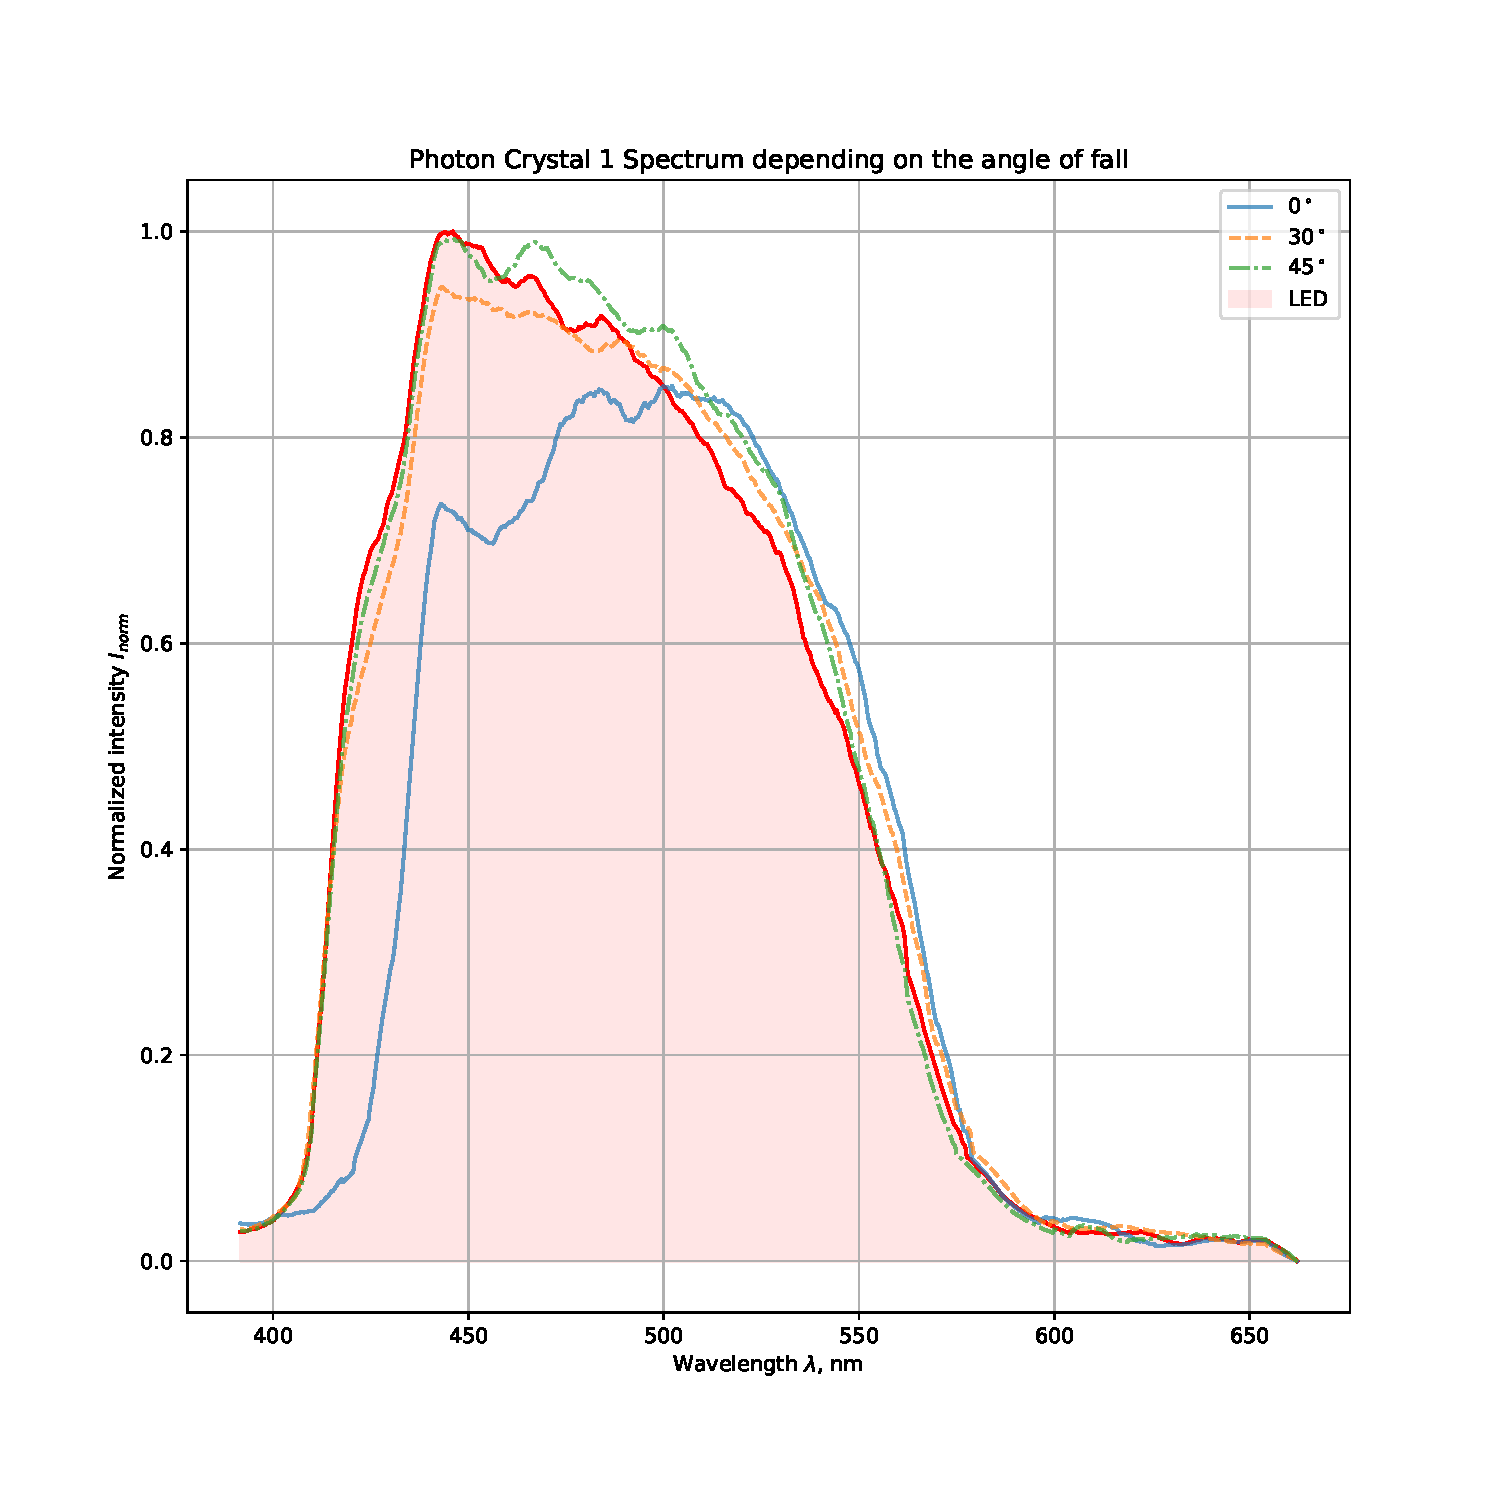
\includegraphics[width=0.7\linewidth]{1.pdf}
	\caption{Спектр после прохождения фотонного кристалла 1}
	\label{fig:1}
\end{figure}

\begin{figure}[H]
	\centering
	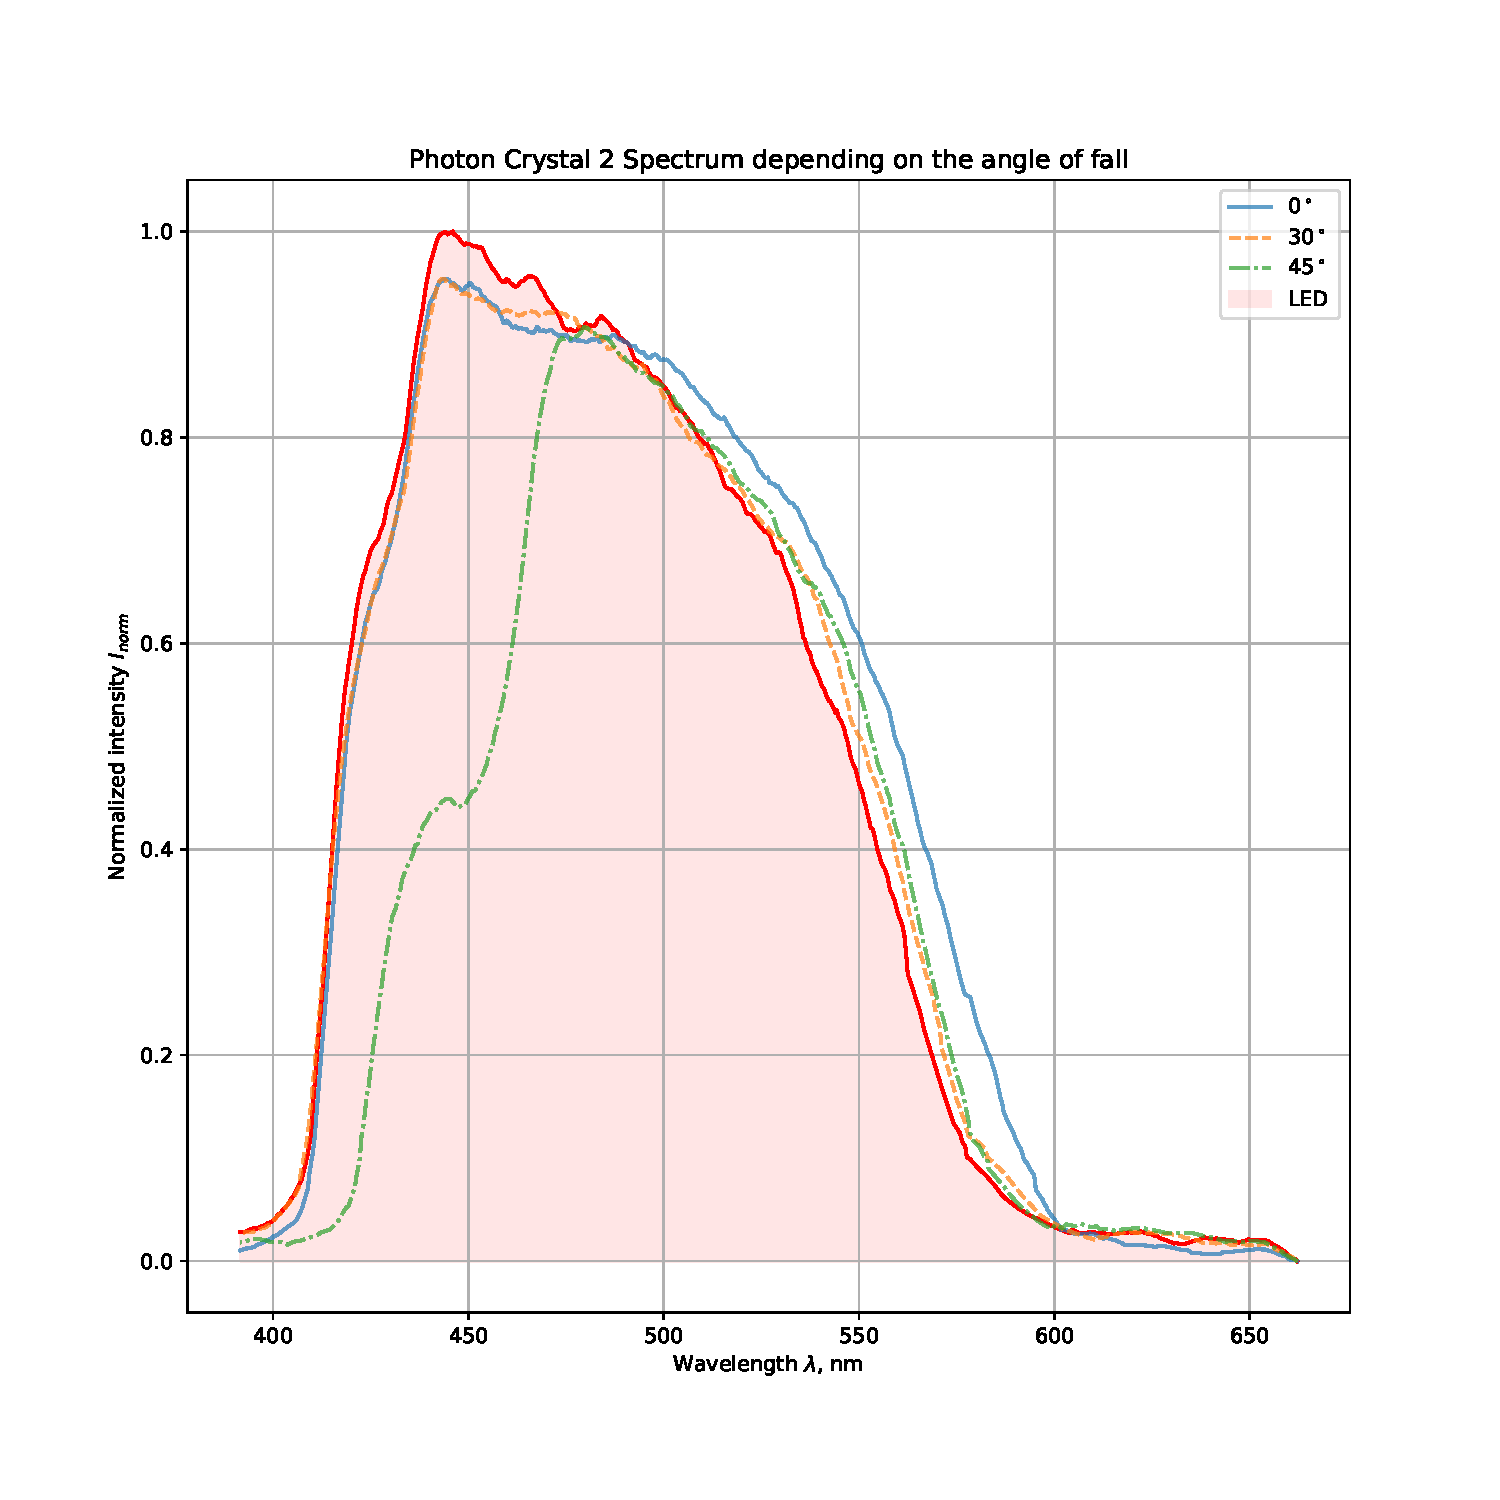
\includegraphics[width=0.7\linewidth]{2.pdf}
	\caption{Спектр после прохождения фотонного кристалла 2}
	\label{fig:2}
\end{figure}

\begin{figure}[H]
	\centering
	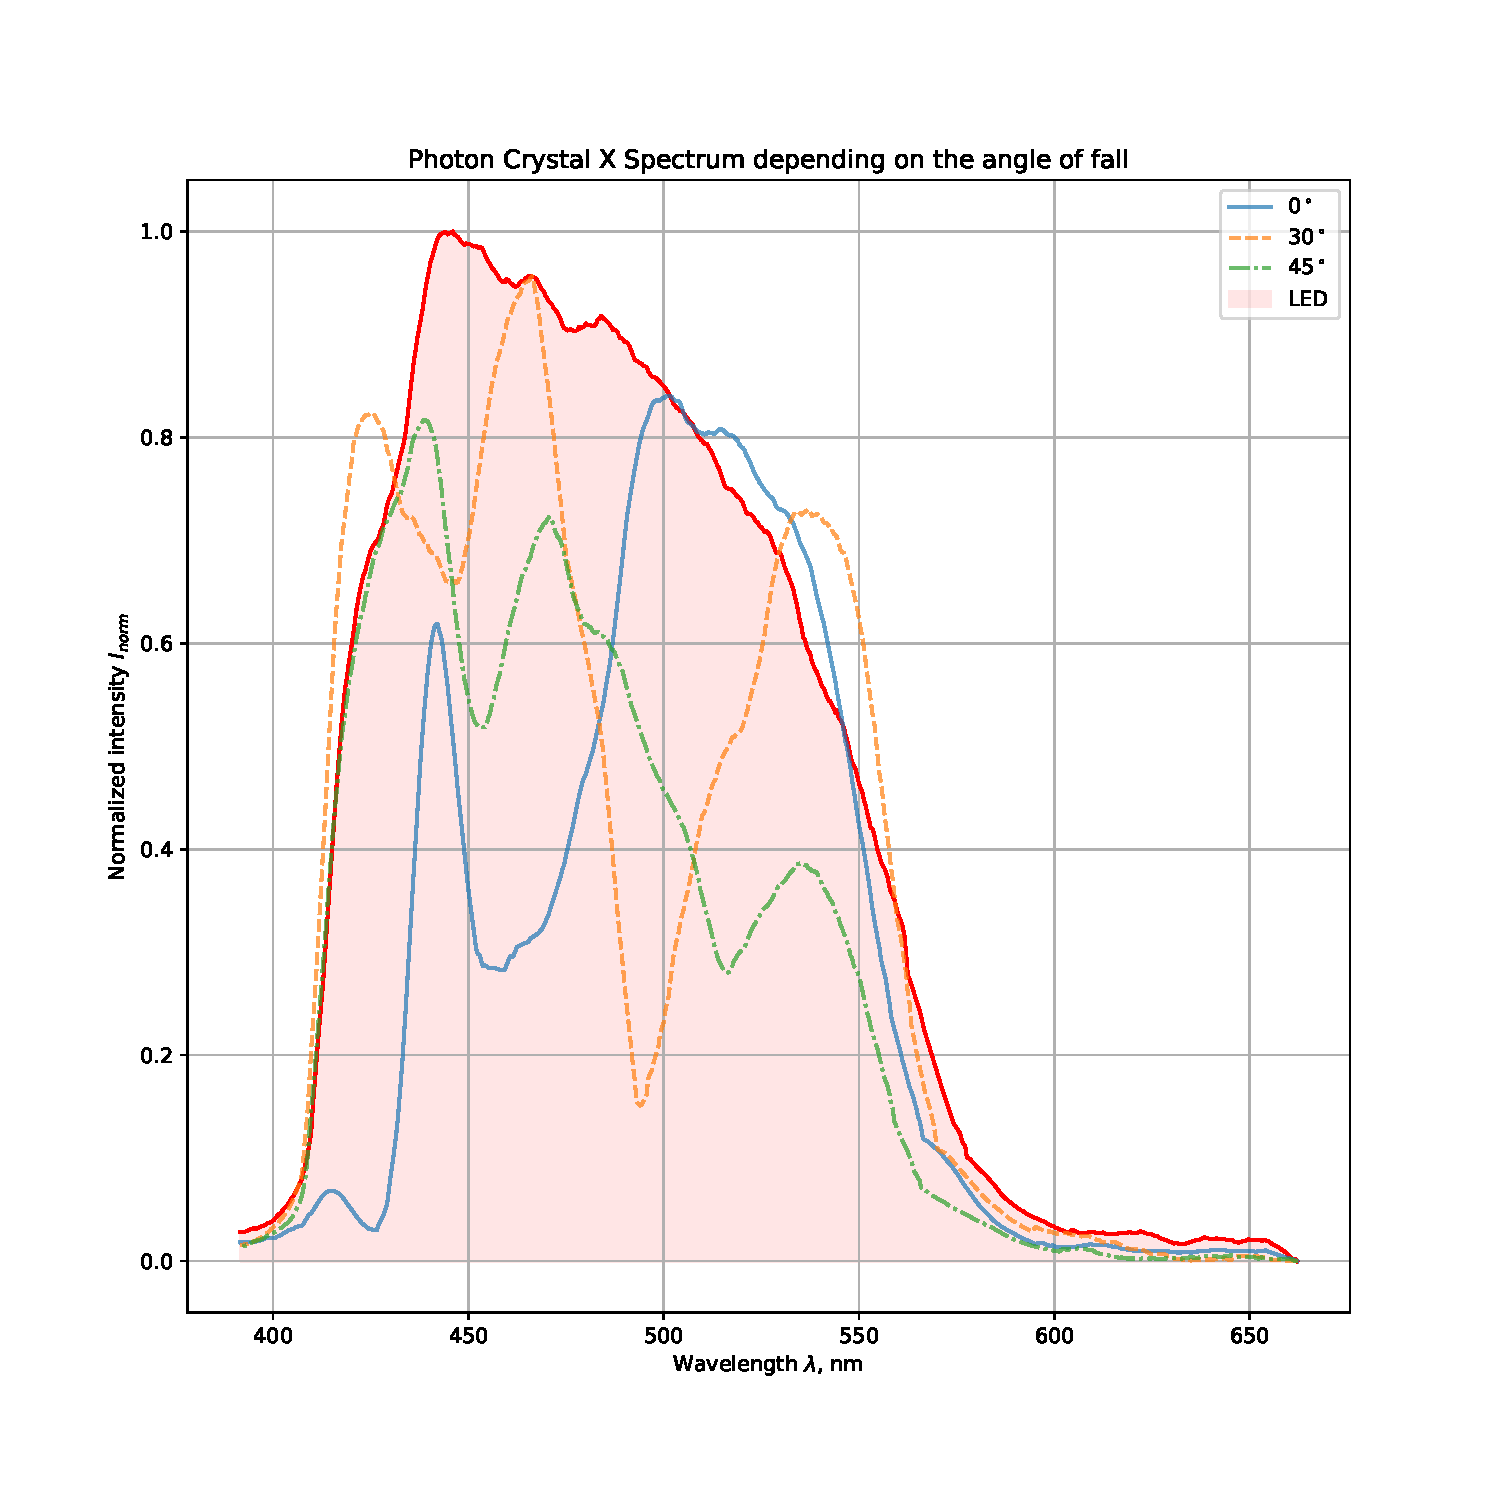
\includegraphics[width=0.7\linewidth]{x.pdf}
	\caption{Спектр после прохождения фотонного кристалла X}
	\label{fig:x}
\end{figure}

\begin{figure}[H]
	\centering
	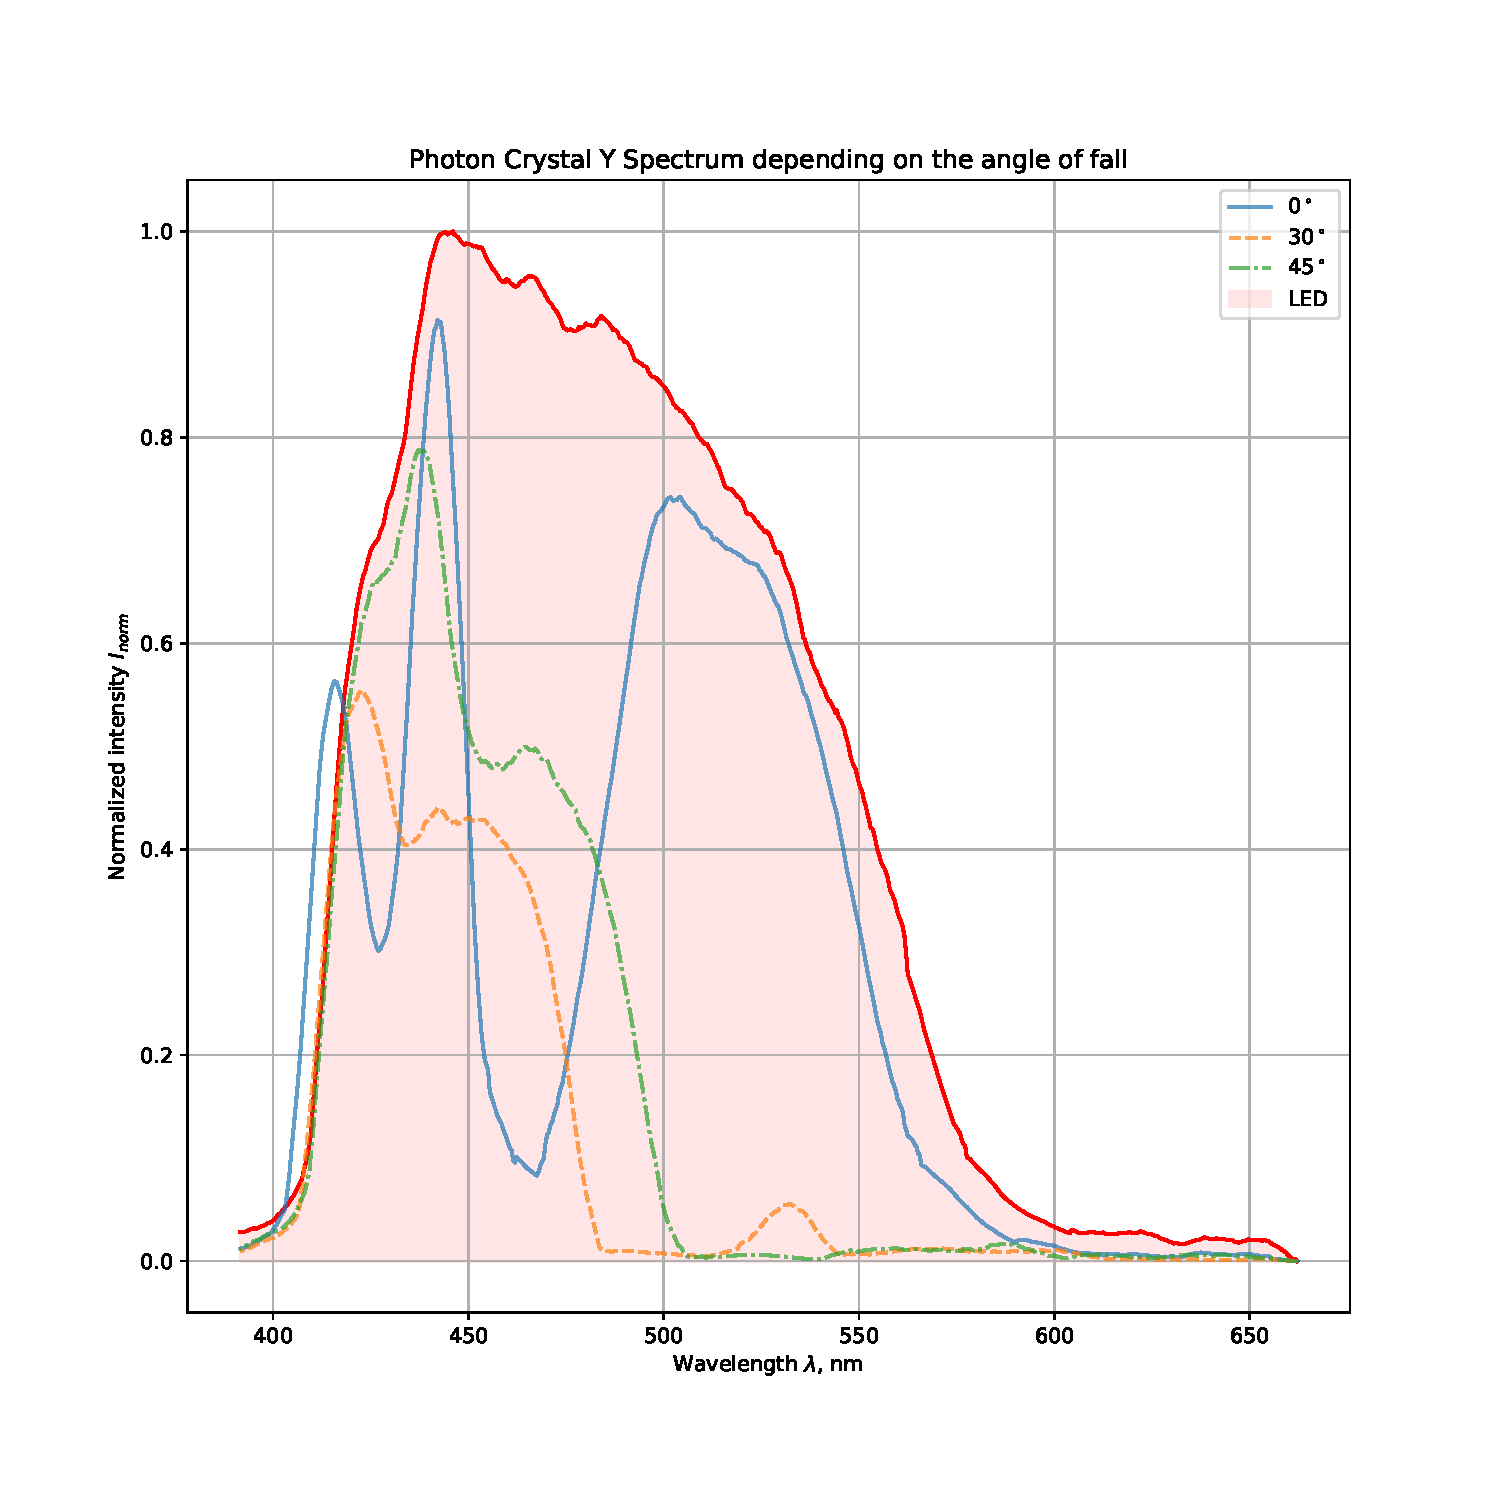
\includegraphics[width=0.7\linewidth]{y.pdf}
	\caption{Спектр после прохождения фотонного кристалла Y}
	\label{fig:y}
\end{figure}

\begin{figure}[H]
	\centering
	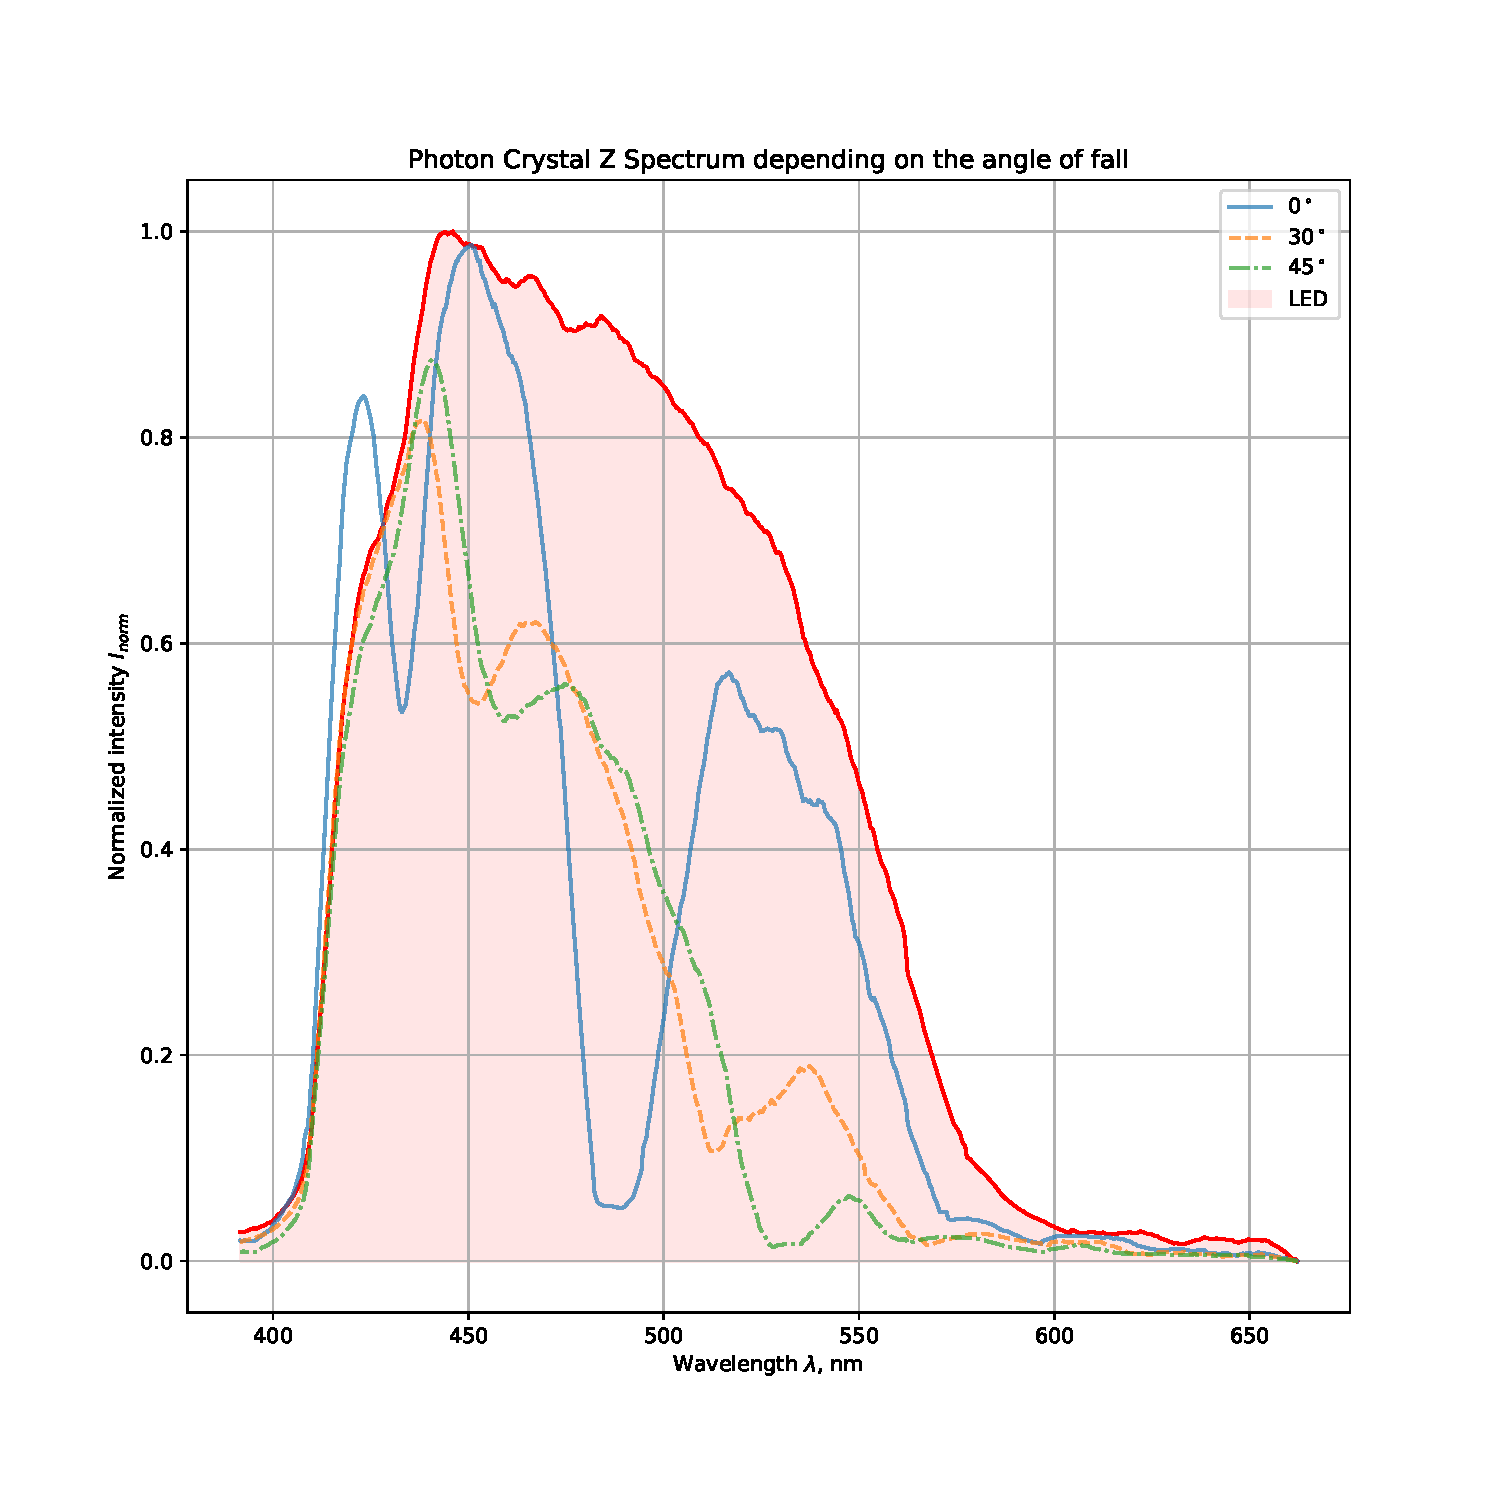
\includegraphics[width=0.7\linewidth]{z.pdf}
	\caption{Спектр после прохождения фотонного кристалла Z}
	\label{fig:z}
\end{figure}

\begin{figure}[H]
	\centering
	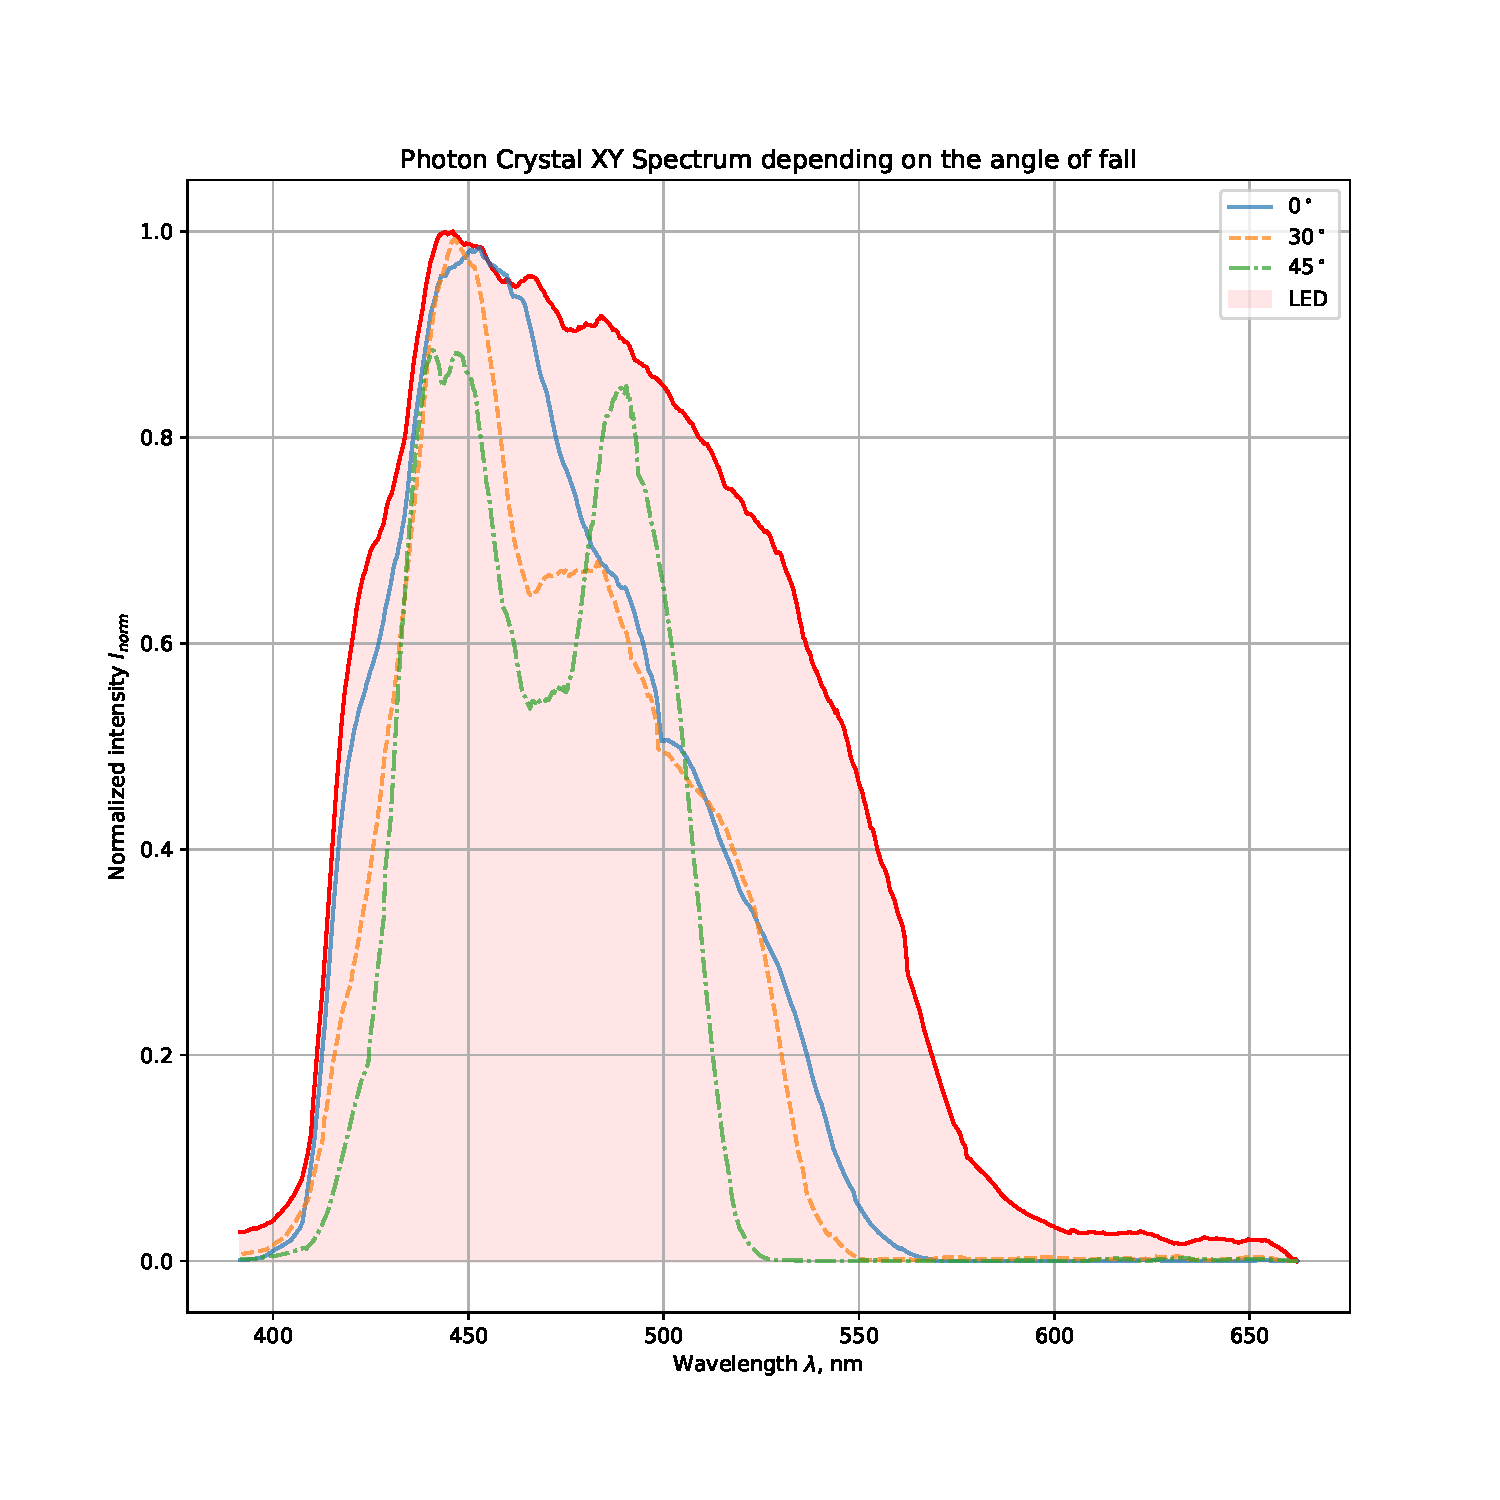
\includegraphics[width=0.7\linewidth]{xy.pdf}
	\caption{Спектр после прохождения фотонных кристаллов XY}
	\label{fig:xy}
\end{figure}

\subsection{Ртутная лампа}

Помимо получения указанных выше спектров была также предпринята попытка получить спектр ртутной лампы. Полученные результаты представлены на рисунке \ref{fig:Hg}. Что можно сказать: в целом видны пики в районе 600~нм и видно начало пиков в районе 400~нм. Тем не менее, разрешение этих пиков, к сожалению, оставляет желать лучшего. Референсный спектр с \href{http://zeiss-campus.magnet.fsu.edu/articles/lightsources/mercuryarc.html}{сайта} приведен на рисунке \ref{fig:hg_ref}.

\begin{figure}[H]
	\centering
	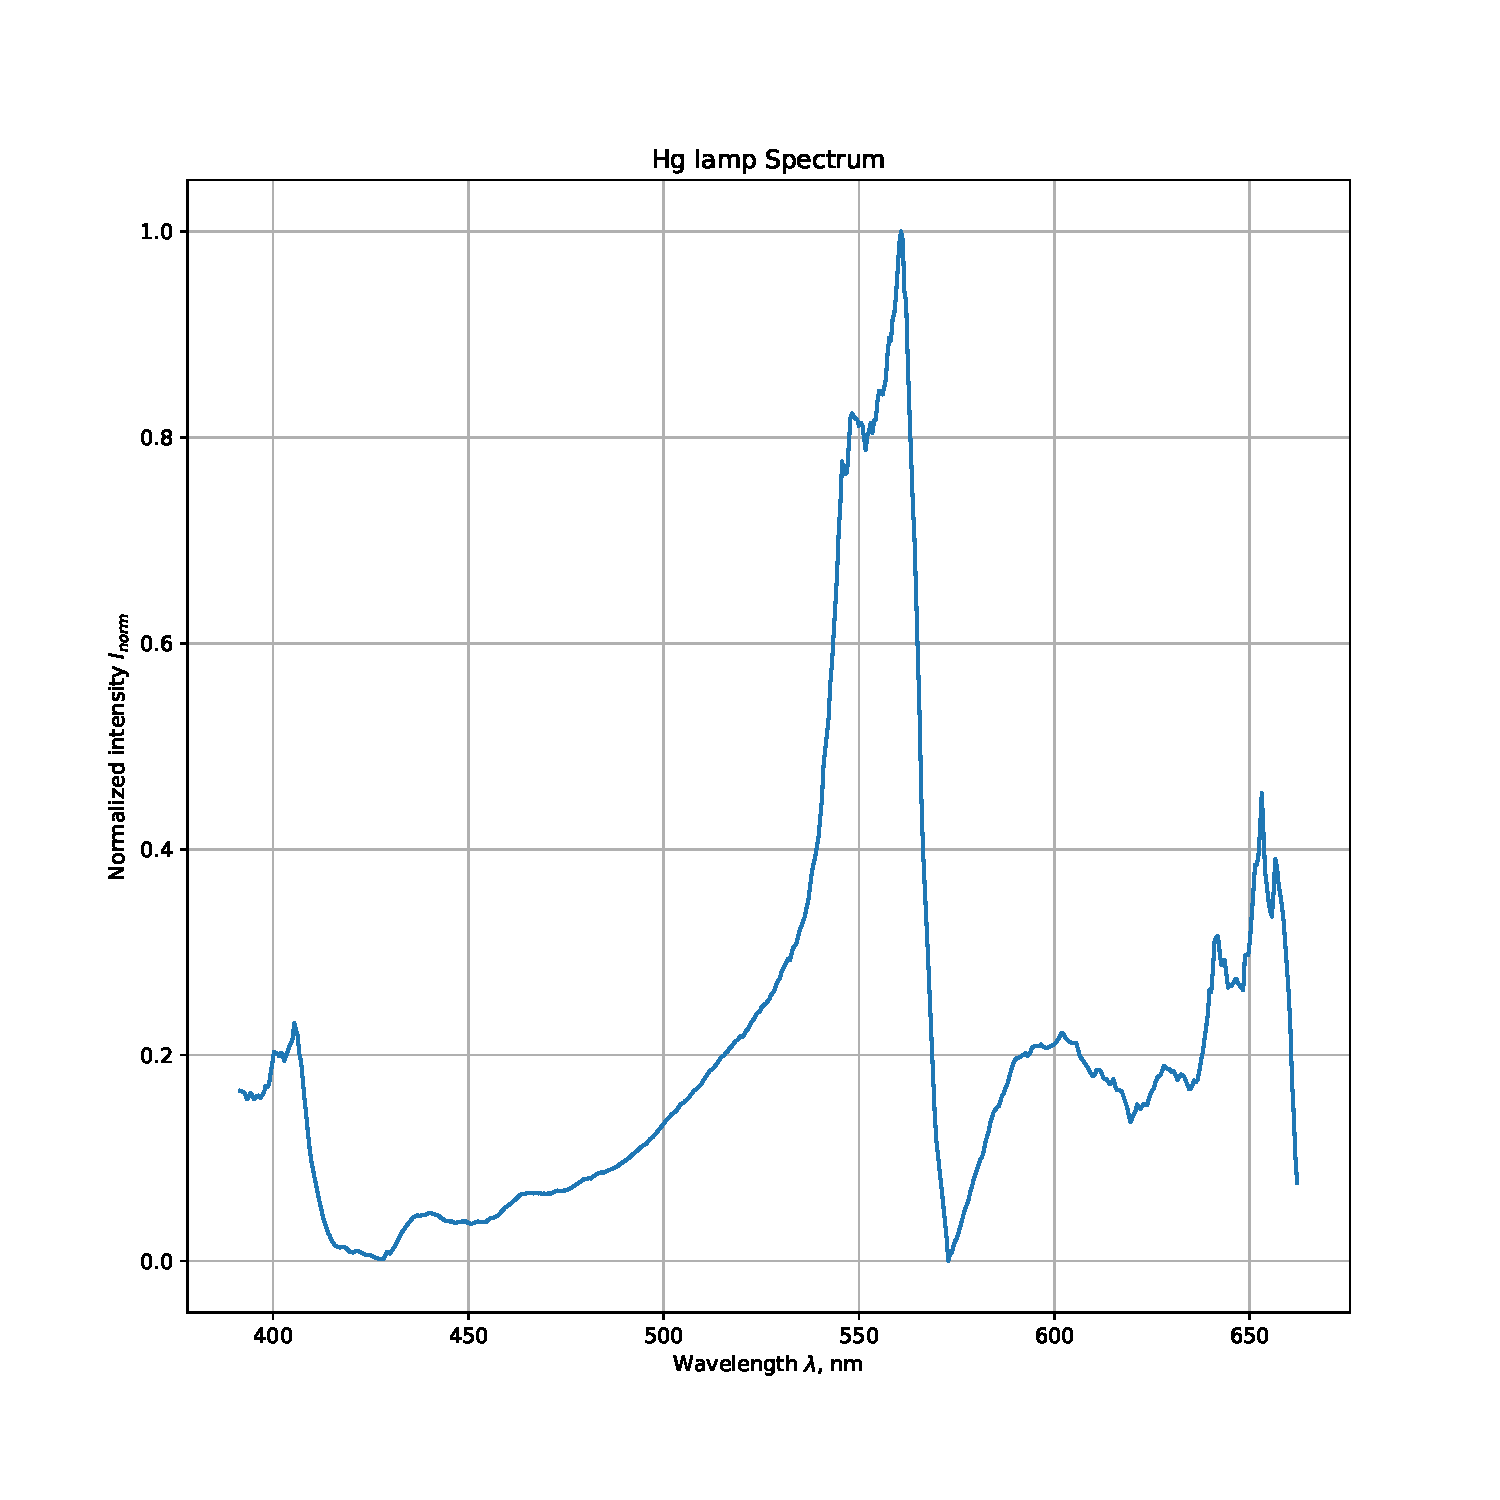
\includegraphics[width=0.7\linewidth]{Hg.pdf}
	\caption{Спектр ртутной лампы}
	\label{fig:Hg}
\end{figure}

\begin{figure}[H]
	\centering
	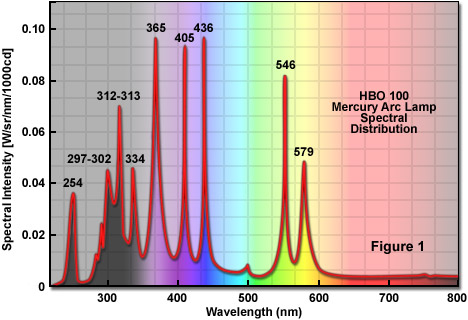
\includegraphics[width=0.7\linewidth]{hg_ref}
	\caption{Референсный спектр ртутной лампы}
	\label{fig:hg_ref}
\end{figure}

\section{Анализ допущенных ошибок (вместо вывода)}

Хотя были получены какие-то данные (местами даже сильно похожие на правильные), ходе эксперимента был допущен ряд ошибок, каждая из которых (в большей или меньшей степени) влияла на качество полученных данных. Приведем некоторые из них:

\begin{itemize}
	\item Использование камеры с RGB-матрицей.
	
	Здесь таится сразу несколько проблем. Во-первых, такая камера является цветной, что в нашем случае является минусом, поскольку, судя по всему, детекторы различных цветов имеют разную чувствительность, из-за чего в основном мы всегда имеем засвет по синему цвету. Кроме того, приходится проводить дополнительные операции по сложению трех сигналов в один. Во-вторых, такая камера имеет малую разрешающую способность. 
	
	Решить это можно использованием, например, ПЗС-линейки, но при проведении экспериментов у нас это не получилось из-за отсутствия рабочего прототипа.
	
	\item Хлипкость и неточность сборки самого спектрометра.
	
	Безусловно, лучшего качества данных можно добиться, если четко фиксировать элементы спектрометра, проводить тщательную юстировку и ни в коем случае даже чуть-чуть не менять конфигурацию спектрометра. В реальности, к сожалению, соединения были местами ненадежными, а юстировка далеко не идеальной. Кроме того, необходимо гораздо тщательнее подбирать расстояния между элементами спектрометра, поскольку это также сильно влияет на качество получаемого спектра.
	
	Конфигурацию спектрометра не менять также не получалось, поскольку необходимо было использовать различные источники, что требовало пусть незначительных, но все же корректировок в установке. В идеале их также необходимо исключить.
	
	\item Изменение интенсивности источника между экспериментами.
	
	Про эту ошибку было упомянуто выше, она не позволяет получить абсолютных значений (хотя при этом позволяет получить форму спектра). Необходимо просто ее не допускать.
	
	\item Наличие фонового светового шума.
	
	Шум необходимо как можно лучше изолировать, в идеале --- проводить измерения в абсолютно темной комнате. Кроме того, необходимо изолировать детектор от попадания на него паразитного света от источника (который не прошел через систему).
	
	
\end{itemize}

\end{document}
